\documentclass[12pt,a4paper]{scrreprt}

\usepackage[utf8]{inputenc}
\usepackage[german]{babel}
\usepackage[T1]{fontenc}
\usepackage{amsmath}
\usepackage{amsfonts}
\usepackage{amssymb}
\usepackage{graphicx}
\usepackage[left=2cm,right=2cm,top=2cm,bottom=2cm]{geometry}

\author{Sebastian Wittmann}
\title{VeraCrypt}
\subtitle{Eine Anleitung zur sicheren Verschlüsselung von privaten Daten}

\begin{document}
\pagenumbering{gobble}
%\maketitle
\begin{titlepage}
\begin{center}
\noindent\rule{470pt}{0.4pt}\par
\vspace{6cm}
{\fontsize{29.86pt}{29.86pt}\selectfont \textbf{Verschlüsselung von Daten}} \par
\vspace{0.5cm}
{\fontsize{17.28pt}{17.28pt}\selectfont Eine Anleitung zur sicheren Verschlüsselung von privaten Daten}\par
\vspace{3cm}
{\fontsize{20.74pt}{20.74pt}\selectfont Sebastian Wittmann} \par
\vspace{2cm}
{\fontsize{14pt}{14pt}\selectfont Version 0.6.0}\par
\vspace{10cm}
{\fontsize{14pt}{14pt}\selectfont 17.03.2019}
\noindent\rule{470pt}{0.4pt}
\end{center}
\end{titlepage}
\pagenumbering{roman}
\tableofcontents

\chapter{Einleitung}
\pagenumbering{arabic}
Die Inhalte aus dem VeraCrypt Theorie Kapitel stammen teilweise aus der englischen Originaldokumentation der offiziellen VeraCrypt Website. Das Ziel dieser Arbeit ist, einen möglichst einfachen Einstieg in die Verschlüsselung von Daten zu bieten.\\

\noindent Egal, ob es sich um vertrauliche Dokumente, oder private Bilder handelt, niemand sollte auf die Idee kommen, diese einfach auf dem heimischen Rechner liegen zu haben. Außerdem kann die Verschlüsselung von Daten das Gedächtnis entlasten, da auch eine Vielzahl von Passwörtern verschlüsselt werden kann. Dabei ist es natürlich von großer Bedeutung, dass dieses eine Passwort, welches für die Verschlüsselung der Daten benutzt wird, besonders sicher ist. Für den Fall, dass nur eine Vielzahl von Passwörtern verschlüsselt werden soll, ist ein Passwortmanager, wie zum Beispiel KeePass 2, eine deutlich bessere Wahl, da diese Software auf diesen Verwendungszweck spezialisiert ist.\\

\noindent Zum Schluss werden noch zwei weitere nützliche Programm vorgestellt. Diese sind Paranoia Text Encryption und S.S.E. File Encryptor. Sie ermöglichen die Verschlüsselung von Texten und einzelnen Dateien. Diese Programme sind eine sehr attraktive Erweiterung, da so auch sehr einfach verschlüsselte Texte über verschiedenste Übertragungsmöglichkeiten zu versenden sind. Damit muss man sich nicht auf den Anbieter der Übertragungsmöglichkeit verlassen, sondern nimmt die Sicherheit selbst in die Hand.\\

\noindent Sollten Fehler in dieser Arbeit gefunden werden, wäre ich sehr dankbar, wenn ich darauf aufmerksam gemacht werde. Das ist entweder über eine kurze Email an mich, oder durch das Erstellen eines Issues auf GitHub möglich. Ich freue mich auch über Feedback!\\

\noindent Email: sebastian.wittmann97zibbo@gmail.com\\

\noindent GitHub: https://github.com/zibbozz/VerschluesselungVonDaten

\part{VeraCrypt}

\chapter{VeraCrypt - Theorie}
Bevor die Abläufe erklärt werden, wird zunächst etwas auf die Theorie eingegangen. Dieses Kapitel ist für Leser, welche sich ebenfalls für die Hintergründe interessieren. Wer direkt loslegen will, kann gerne direkt zur Praxis springen. Dort kann alles befolgt werden, ohne sich die Theorie durchgelesen zu haben.

\section{Was ist VeraCrypt?}
VeraCrypt ist eine Software, welche es einem Benutzer ermöglicht seine privaten Daten mit einem Passwort zu verschlüsseln. Es bietet die Möglichkeit Container-Dateien zu erstellen, welche als eigenes Laufwerk eingebunden werden können. Das ist aber noch nicht alles. VeraCrypt bietet außerdem die Möglichkeit ein ganzes Laufwerk oder etwa einen USB Stick zu verschlüsseln. Wer wirklich sicher gehen möchte, kann sogar seinen kompletten Rechner verschlüsseln. Dafür installiert VeraCrypt einen eigenen Bootloader, welcher den Benutzer beim Start des Rechners auffordert, ein Passwort einzugeben. Nur wenn dieses Passwort korrekt ist, wird das Betriebssystem entschlüsselt und der Rechner startet wie gewohnt. \\

\noindent Ein weiterer besonderer Punkt bei VeraCrypt ist, dass es die Möglichkeit gibt, einen versteckten Container, ein verstecktes Laufwerk oder sogar ein verstecktes Betriebssystem zu erstellen. Das bedeutet, dass je nachdem, welches Passwort eingegeben wird, entweder der normale Inhalt oder der geheime Inhalt angezeigt wird. Das ist in Situationen nützlich, in denen ein Angreifer von dem Container weiß und den Benutzer zwingt, den Container zu entschlüsseln. Der Angreifer kann nicht wissen, dass der geheime Inhalt existiert.

\section{Benötigte Rechte}
Da VeraCrypt einen eigenen Treiber besitzt, der es ermöglicht, die Container oder Laufwerke einzubinden, muss es installiert werden, um den vollen Funktionsumfang zu bieten. Es gibt jedoch auch einen Portable-Modus. Dieser kann nur benutzt werden, wenn der Benutzer Administratorrechte besitzt. Sollte VeraCrypt auf dem Rechner installiert sein, kann auch ein Benutzer ohne Administratorrechte das Programm benutzen.

\section{Verschlüsselungsalgorithmen}
VeraCrypt bietet in der aktuellen Version (1.23) fünf verschiedene Verschlüsselungsmethoden. Dazu kommen noch Kaskaden dieser Methoden, wodurch es insgesamt 15 Möglichkeiten der Verschlüsselung gibt. Anhand eines Benchmarks kann festgestellt werden, welche Algorithmen besonders sicher sind. Sicher bedeutet in diesem Fall, dass die Daten langsam verschlüsselt werden. Können die Daten nur langsam verschlüsselt werden, dauert die Entschlüsselung ebenfalls lange.\\

\begin{figure}[t]
\begin{center}
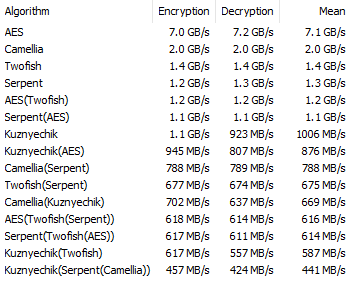
\includegraphics[width=250pt]{media/encryptionBenchmark.png}
\caption{Benchmark Verschlüsselungsalgorithmen}
\label{encbench}
\end{center}
\end{figure}

\noindent Dieser Benchmark wurde auf einem System mit einem Intel i7-7700K@4,20Ghz durchgeführt. Die Buffer Size wurde auf 1 GB gestellt, um geschätzte Werte so weit es möglich ist, zu vermeiden. Anhand der Grafik ist zu sehen, dass die Kaskade aus Kuznyechik, Serpent und Camellia eine gute Wahl wäre.

\section{Hardwarebeschleunigung}

Der AES Algorithmus wird von manchen Prozessoren nativ unterstützt. Das bedeutet, dass die Ver- und Entschlüsselung mit diesem Algorithmus etwa 4-8 mal so schnell ist, wie mit einem Prozessor, der diesem Algorithmus nicht nativ unterstützt. Es kann entweder im Internet nachgelesen werden, ob die verbaute CPU den AES-NI Befehlssatz unterstützt, oder einfach im VeraCrypt Benchmark am unteren Rand abgelesen werden. VeraCrypt verwendet jedoch nicht alle Befehle des AES-NI Befehlssatzes, sondern nur die Hauptbefehle. Die Erzeugung der Schlüssel wird stets durch die Software und nicht direkt durch den Prozessor bewerkstelligt.

\begin{figure}[h!]
\begin{center}
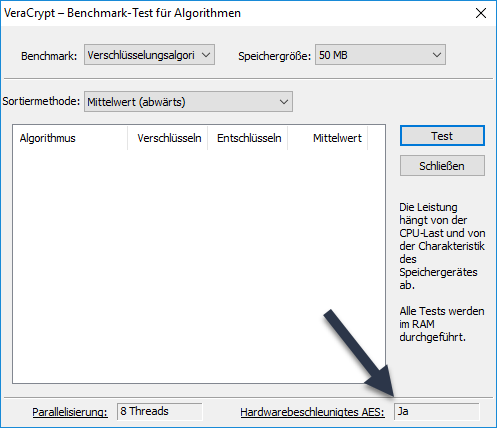
\includegraphics[width=230pt]{media/aessupport.png}
\caption{Unterstützung für die Hardwarebeschleunigung}
\label{aessupport}
\end{center}
\end{figure}

\newpage

\section{Hash-Algorithmen}
Die Hash-Algorithmen sind dafür verantwortlich, dass das Passwort des Benutzers auf eine bestimmte Länge gebracht wird, damit es von den Verschlüsselungsalgorithmen verwendet werden kann. Auch hier kann ein Benchmark durchgeführt werden, um die Geschwindigkeit der Algorithmen zu sehen.

\begin{figure}[h]
\begin{center}
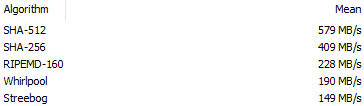
\includegraphics[width=250pt]{media/hashBenchmark.png}
\caption{Benchmark Hash-Algorithmen}
\label{hashbench}
\end{center}
\end{figure}

\section{Der Random Number Generator}
Der Random Number Generator wird von VeraCrypt verwendet, um den Masterschlüssel, den sekundären Schlüssel, Salt und die Keyfiles zu generieren. Dieser Generator erschafft zufällige Werte im Arbeitsspeicher, damit das Programm damit arbeiten kann. Der erschaffene Pool ist 320 Bytes groß. Um diese zufälligen Werte zu erstellen, verwendet der Generator folgende Quellen:

\begin{itemize}
\item Mausbewegungen
\item Tastenanschläge
\item Mac OS X und Linux: Werte der eigenen Generatoren \textit{/dev/random} und \textit{/dev/urandom}
\item Windows: Windows CryptoAPI
\item Windows: Netzwerkschnittstelle (NETAPI32)
\item Windows: Verschiedene Win32 Handles, Zeitvariablen und Zähler
\end{itemize}

\noindent Bevor jedoch ein Wert aus den oben genannten Quellen in den Pool geschrieben wird, teilt VeraCrypt den Wert in einzelne Bytes auf. Diese Bytes werden dann mit einer Modulo $2^8$ Rechenoperation in den Pool geschrieben. Der Pool besitzt einen Zeiger, der nach jedem Schreibvorgang einen Byte weiter springt, um dort das nächste Byte hinzuschreiben. Wenn der Zeiger das Ende des Pools erreicht, so springt dieser wieder an den Anfang des Pools und fängt dort an die Werte zu überschreiben. Nach jedem 16. Byte, das geschrieben wurde, wird auf den kompletten Pool eine Funktion angewendet, der die Werte noch einmal mischt. Dadurch wird eine Rekonstruktion des Pools erst recht unmöglich.

\section{Sichere Passwörter}
Sämtliche Verschlüsselungsmethoden bringen nicht sehr viel, wenn das verwendete Passwort nicht sicher ist. Je komplizierter der Algorithmus ist, umso länger dauert ein Bruteforce Angriff, doch bei einem einfachen Passwort wie \textit{12345} dauert es selbst bei der langsamsten Kaskade nicht sehr lange, bis das Passwort geknackt ist.
\subsection{Top 10 der meistverwendeten Passwörter}
Sollte das eigene Passwort in der folgenden Liste auftauchen, bitte ich darum, dieses Passwort so schnell wie möglich zu ändern. Der Grund dafür ist, dass bei einem Angriff meistens Passwortlisten verwendet werden und somit dieses Passwort in weniger als einer Sekunde geknackt wird.

\begin{enumerate}
\item 123456
\item password
\item 12345678
\item qwerty
\item 12345
\item 123456789
\item letmein
\item 1234567
\item football
\item iloveyou
\end{enumerate}

\subsection{Die Wahl eines guten Passworts}
Auf vielen Websites gibt es Hinweise, was ein Passwort erfüllen sollten. An diese Richtlinien sollte man sich wirklich halten. Bei einem Passwort sollten folgende Kriterien zutreffen:\\

\begin{itemize}
\item Groß- und Kleinbuchstaben enthalten
\item Zahlen enthalten
\item Sonderzeichen enthalten
\item Keine Leerzeichen
\item Keine Wörter, die in einem Wörterbuch zu finden sind
\item Keine aufeinanderfolgenden Zahlen oder Buchstaben
\item Großen Abstand der Tasten auf der Tastatur
\item Gute Passwortlänge
\end{itemize}

\subsection{Entropie eines Passworts}
Die Entropie eines Passworts beschreibt den Informationsgehalt und wird in Bits angegeben. Je höher die Entropie eines Passworts, umso besser für den Benutzer. Die Entropie eines Passworts lässt sich mit einer ziemlich einfachen Formel berechnen.\\

\noindent $H = L\times\log_2N$\\

\noindent H steht hierbei für die Entropie, L ist Anzahl der Zeichen des Passworts und N ist die Anzahl der möglichen Zeichen. Wenn das Passwort beispielsweise nur aus Kleinbuchstaben besteht, besitzt N den Wert 26. Für die Entropie gilt im Allgemeinen folgendes:\\

\begin{itemize}
\item < 28 bits = Sehr schwach, hält unerfahrene Nutzer fern
\item 28-35 bits = Schwach, sollte die meisten Leuten fernhalten
\item 36-59 bits = In Ordnung, für Onlinezwecke verwendbar
\item 60-127 bits = Stark, kann für wichtige Zwecke (PayPal) verwendet werden
\item > 128 bits = Sehr stark, meistens zu viel des Guten
\end{itemize}

\subsection{Dauer bis ein Passwort geknackt wird}
Es ist zu bedenken, dass folgende Zahlen im besten Fall zutreffen, wenn das richtige Passwort als letztes getestet wird. Es kann also etwa die Zahl geteilt durch zwei genommen werden, um eine realistische Zahl zu bekommen. Bei besonders viel Pech kann natürlich auch ein sehr starkes Passwort beim ersten Versucht geknackt werden.\\

\begin{figure}[h]
\begin{center}
\begin{tabular}{c|c|c|c|c|c|c}
Entropie&10 Tsd v/s&1 Mio v/s&1 Mrd v/s&100 Mrd v/s&1 Bio v/s&100 Bio v/s\\
120&$\infty$ &$\infty$ &$\infty$ & 421 Brd J & 42 Brd J & 421 Bio J\\
110&$\infty$ &$\infty$ & 41 Brd J & 411 Bio J & 42 Bio J & 411 Mrd J\\
100&$\infty$ & 40 Brd J & 40 Bio J & 402 Mrd J & 40 Mrd J & 402 Mio J\\
90&3.9 Brd J & 39 Bio J & 39 Mrd J & 392 Mio J & 39 Mio J & 392 Tsd J\\
80&3.8 Bio J & 38 Mrd J & 38 Mio J & 383 Tsd J & 38 Tsd J & 383 J\\
70&3.7 Mrd J & 37 Mio J & 37 Tsd J & 374 J & 37 J & 4.5 M\\
60&3.7 Mio J & 37 Tsd J & 37 J & 4.4 M & 13 T & 3.2 S\\
50&3.6 Tsd J & 36 J & 13 T & 3.1 S & 19 Min & 11 Sek\\
40&3.5 J & 13 T & 18 Min & 11 Sek & 1.1 Sek & 0.011 Sek
\end{tabular}
\end{center}
\caption{v/s = Versuche pro Sekunde; J = Jahre; M = Monate; T = Tage; S = Stunden; Min = Minuten; Sek = Sekunden}
\end{figure}

\noindent Eine komplette Tabelle befindet sich im Anhang.

\newpage

\section{PIM}
PIM (Personal Iterations Multiplier) bestimmt, wie oft ein Algorithmus die Daten bearbeitet. Ein hoher PIM erhöht zwar die Sicherheit, sorgt jedoch auch dafür, dass das Einbinden deutlich länger dauert. Wurde der PIM vom Benutzer bei der Erstellung eines Containers angegeben, muss dieser auch beim Einbinden wieder eingegeben werden. Er dient also zugleich als ein zweites Passwort. \\

\noindent Der PIM bestimmt jedoch nicht die exakte Anzahl der Durchläufe. Für die Anzahl der Durchläufe gibt es zwei Formeln:

\begin{itemize}
\item Systemverschlüsselung nicht mit SHA-512 oder Whirlpool:\\ $PIM\times 2048$
\item Systemverschlüsselung mit SHA-512 oder Whirlpool, Laufwerke und Container:\\ $15000+(PIM\times 1000)$
\end{itemize}

\noindent Der PIM kann nicht beliebig klein gewählt werden, wenn ein Passwort mit weniger als 20 Zeichen gewählt wurde, um ein Minimum an Sicherheit zu bieten. Für eine Systemverschlüsselung nicht mit SHA-512 oder Whirlpool beträgt das Minimum und zugleich der Standard \textbf{98} und bei einer Systemverschlüsselung mit SHA-512 oder Whirlpool, Laufwerken und Containern beträgt es \textbf{485}.

\section{Keyfiles}
Durch die Verwendung von Keyfiles kann für zusätzliche Sicherheit gesorgt werden, denn diese können ähnlich wie der PIM zusätzlich zum Passwort verwendet werden. Es können beliebig viele Keyfiles für ein Volume eingetragen werden, jedoch muss bei der Entschlüsselung jede angegebene Datei vorhanden sein, da sonst eine Entschlüsselung unmöglich ist. \\

\noindent VeraCrypt benutzt die ersten 1024 kilobytes einer Datei, um daraus den Schlüssel zu bilden. Daher sollten die Dateien nach der Registrierung auch nicht mehr geändert werden. Es wird empfohlen Dateien zu verwenden, die komprimiert wurden, da die Bits diese Dateien zufälliger sind. Beispiele für komprimierte Dateien sind .mp3, .jpg, .zip usw. \\

\noindent Das Programm bietet sogar die Möglichkeit komplett zufällige Dateien zu erzeugen, die dann als Keyfiles dienen können. Diese Funktion ist unter Extras unter dem Namen \textbf{Schlüsseldatei(en) generieren} zu finden. Alternativ findet man diese Option bei der Erstellung eines Volumes, wenn man die Einstellungen bezüglich der Keyfiles anpasst.

\section{Glaubhafte Abstreitbarkeit}
VeraCrypt bietet bereits zwei große Bestandteile, um die Existenz eines Containers zu bestreiten (Gleiches gilt für Laufwerke und Betriebssysteme). Diese sind:

\begin{enumerate}
\item Verstecke Container
\item Komplett zufällig aussehende Daten eines verschlüsselten Containers
\end{enumerate}

\noindent Wie bereits erwähnt, kann niemand wissen, dass ein versteckter Container überhaupt existiert. Dazu kommt, dass es auch wirklich niemand nachweisen kann. Es gibt keine Zeichenfolgen in einem verschlüsselten Container, welche darauf hinweisen, dass dieser einen versteckten Teil beinhaltet. Aus diesem Grund sollte der Benutzer sehr vorsichtig sein, wenn der normale Container mit Daten befüllt wird. Werden zu viele Daten in diesem Container gelegt, werden die Daten des geheimen Containers einfach überschrieben. Das gehört zu VeraCrypt's Politik. Laut VeraCrypt sollen Daten lieber zerstört werden, als in falsche Hände zu geraten.

\section{Sicherheitsanforderungen und Vorsichtsmaßnahmen}
Sollten nicht nur die Fotos aus dem letzten Urlaub verschlüsselt werden, sondern beispielsweise die größten Firmengeheimnisse, so sollten einige Aspekte beachtet werden, damit es niemanden möglich ist, trotz Verschlüsselung an die Daten zu kommen. Dazu gehört nicht nur ein gutes Passwort, sondern im Besten Fall die Geheimhaltung der Nutzung von VeraCrypt. Sollte ein Angreifer in das Netzwerk eingedrungen sein, weiß er noch lange nicht, wo die geheimen Daten liegen und er weiß nicht sofort, dass VeraCrypt für die Verschlüsselung verwendet wurde.

\subsection{Datenlecks}
Sobald ein VeraCrypt Container eingebunden wird, können das Betriebssystem oder andere Anwendungen von Drittanbietern unverschlüsselte Informationen zu den im Container gespeicherten Daten, wie beispielsweise Dateinamen oder Speicherorte, auf der Festplatte hinterlassen. Außerdem können unverschlüsselte temporäre Dateien durch Programme entstehen, welche mit dem Auswurf des Containers nicht verschlüsselt werden. \\

\noindent Ein weiterer Schwachpunkt ist, dass Windows automatisch Namen und Speicherorte geöffneter Dateien in der Registry speichert. Diese können unter folgendem Pfad gefunden werden: \\

\textit{HKEY\_{}USERS\textbackslash USERID\textbackslash Software\textbackslash Microsoft\textbackslash Windows\textbackslash Shell\textbackslash} \\

\noindent Um an die Userid zu kommen, kann unter folgendem Eintrag nachgeschaut werden: \\

\textit{HKEY\_{}LOCAL\_{}MACHINE\textbackslash Software\textbackslash Microsoft\textbackslash Windows NT\textbackslash CurrentVersion\textbackslash ProfileList\textbackslash} \\

\noindent Dort können alle Einträge durchgegangen werden und der richtige Eintrag durch den Schlüssel \textit{ProfileImagePath} identifiziert werden. \\

\noindent Windows bietet noch ein Datenleck und dieses hängt mit dem NTFS Dateisystem zusammen. Seit Windows 8 wird beim Einbinden eines NTFS Containers ein Event 98 in das Systemereignisprotokoll geschrieben. In diesem Protokoll kann der Name des Containers eingesehen werden. Dies kann umgangen werden, indem der Container als Wechselmedium eingebunden wird. \\

\noindent Um Datenlecks allgemein zu vermeiden können folgende Hinweise beachtet werden:

\begin{itemize}
\item Wenn die Existenz des Containers nicht geleugnet werden muss:
\begin{itemize}
\item Es sollte die Systempartition verschlüsselt werden, damit auch sämtliche Logs verschlüsselt werden.
\item Es sollte ein Live-Betriebssystem geladen werden. Dadurch werden die Logs erst gar nicht gespeichert, da sich das komplette Betriebssystem im Arbeitsspeicher befindet.
\end{itemize}
\item Wenn die Existenz des Containers geleugnet werden muss:
\begin{itemize}
\item Es sollte ein verstecktes Betriebssystem neben dem eigentlichen Betriebssystem erstellt werden, damit die Logs verschlüsselt und die Existenz dieser Logs geleugnet werden kann.
\item Es kann ebenfalls ein Live-System verwendet werden, da alle Daten verschwinden. Daten im Arbeitsspeicher sind nach dem Ausschalten des Rechners gelöscht und können im Normalfall nicht wiederhergestellt werden.
\end{itemize}
\end{itemize}

\subsection{Auslagerungsdatei}
Die Auslagerungs-, Paging-, oder auch Swap-Datei wird von Windows erzeugt, wenn Daten, welche in den Arbeitsspeicher geladen werden sollen, nicht mehr in diesem reinpassen. Da diese Daten nicht einfach verworfen werden können, da dies sonst zu Abstürzen führend kann, werden diese Daten auf der Festplatte abgelegt. Dieser Vorgang kann nicht verhindert werden, da es eine Eigenschaft der Betriebssysteme ist. Dieses Problem kann dennoch vermieden werden, indem die Systempartition verschlüsselt wird und selbst Rückstände der Auslagerungsdateien nicht mehr lesbar sind.

\subsection{Ruhezustandsdatei}
Bei der Ruhezustandsdatei oder auch Hibernation File tritt ein ähnliches Problem auf, wie bei der Auslagerungsdatei. Diese Datei wird vom Betriebssystem erzeugt, wenn es nicht komplett herunterfährt, sondern für einen Schnellstart konfiguriert ist oder einfach in den Ruhemodus geht. In der Ruhezustandsdatei werden alle Inhalte des Arbeitsspeicher geladen, damit diese beim erneuten Start des Systems einfach von der Festplatte wieder in den Arbeitsspeicher geladen werden können. Auch dieses Problem kann durch eine Verschlüsselung der Systempartition verhindert werden. Es kann aber auch einfach der Schnellstart unter den Energieeinstellungen deaktiviert werden.

\subsection{Speicherabbilddateien}
Speicherabbilddateien werden beispielsweise bei einem Bluescreen gespeichert. Auch diese enthalten Teile des Arbeitsspeichers, welche auf der Festplatte landen. Diese Dateien können unzugänglich gemacht werden, indem die Systempartition verschlüsselt wird.

\subsection{Physische Sicherheit}
Das System kann so stark verschlüsselt werden, wie man will, doch wenn ein Angreifer direkten Zugriff auf das System hat, kann dieser durch Änderungen an der Hardware an das Passwort für die Verschlüsselung kommen und diese wird dadurch wirkungslos. Es ist generell ratsam, niemals einen fremden Rechner zur Ver- oder Entschlüsselung zu verwenden.

\subsection{Malware}
Ein Angreifer kann bereits vor der Verschlüsselung Zugriff auf das System haben, indem sich eine beliebige Art von Malware auf dem Rechner befindet. Diese könnte das Passwort bereits bei der ersten Eingabe abfangen und der Angreifer kann ungehindert auf die Daten zugreifen. Wenn der Benutzer besonders sicher vorgehen möchte, ist es zu empfehlen die Daten nur auf einem Rechner zu ver- und entschlüsseln, der frisch aufgesetzt wurde und keinen Internetzugriff hat. Außerdem sollten USB Sticks, welche an diesem Rechner angeschlossen werden, an keine anderen Rechner angeschlossen werden.

\subsection{Mehrere Benutzer an einem Rechner}
Es kann öfter vorkommen, dass an einem Rechner mehrere Benutzer existieren. Es ist anzumerken, dass VeraCrypt Container für alle Benutzer auf dem Rechner sichtbar sind. Die Inhalte können trotzdem durch das NTFS Berechtigungssystem geschützt werden. Dies ist jedoch nur möglich, wenn der Container nicht als Wechselmedium eingehängt wurde.

\subsection{Wahl eines starken Passworts}
Die Wahl eines starken Passworts ist essenziell, da ein Angreifer sonst ein sehr leichtes Spiel hat. Ein gutes Passwort enthält keine Namen, Geburtsdaten oder sonstige persönliche Dinge. Außerdem sollte ein Passwort immer aus Groß- und Kleinbuchstaben, Zahlen und Sonderzeichen bestehen. Eine Länge von mindestens 20 Zeichen ist ein guter Anfang. VeraCrypt weist den Benutzer darauf hin, wenn das Passwort zu kurz sein sollte. Diese Meldung kann ignoriert werden, sollte aber im realen Einsatz nicht geschehen.

\subsection{Schlüsseldateien}
Um Brute-Force Angriffe auf eine Schlüsseldatei stark zu erschweren, sollte die Dateigröße mindestens 30 Bytes betragen. Es ist naheliegend, den Generator zu verwenden, den VeraCrypt mitliefert, da dieser auch für die nötige Entropie sorgt.

\subsection{Benennung des Containers}
Der Name eines Containers kann bereits stark zur Sicherheit beitragen. Er sollte natürlich nicht einen Namen tragen wie \textit{Geheim} oder \textit{HierSindAlleMeineDaten}, sondern logischerweise etwas getarnt werden. Ein erster Schritt wäre, eine Endung an die Datei zu hängen (natürlich nicht .hc, da es die Standard-Endung ist). Es ist jedoch davon abzuraten, Endungen wie \textit{.dll} oder sogar \textit{.exe} zu verwenden, da diese für große Probleme sorgen könnten. Eine gute Wahl wäre eine Endung, bei der niemand auf die Idee kommt, diese Datei zu öffnen, da den Inhalt eh keiner lesen kann. Für Benutzer, die auf ihrem Rechner Spiele spielen, wäre beispielsweise ein Dateiname wie \textit{profile003.sav} eine sehr gute Tarnung.

\chapter{VeraCrypt - Praxis}
In diesem Kapitel geht es um die reine Durchführung um so schnell wie möglich an das Ziel zu kommen. Es wird nur das nötigste erklärt, da die tiefgehenden Erklärungen im Kapitel zweiten Kapitel \textit{Theorie} zu finden sind.

\section{Sprache umstellen}
Da manche Benutzer nicht mit den englischen Begriffen problemlos zurechtkommen, bietet das Programm die Möglichkeit, die Sprache umzustellen. Dazu muss unter \textbf{Settings} der Menüpunkt \textbf{Language...} angeklickt werden. Dort kann der Benutzer die gewünschte Sprache wählen.\\

\noindent \underline{In den folgenden Anleitungen werden die deutschen Begriffe verwendet.}

\begin{figure}[h]
\begin{center}
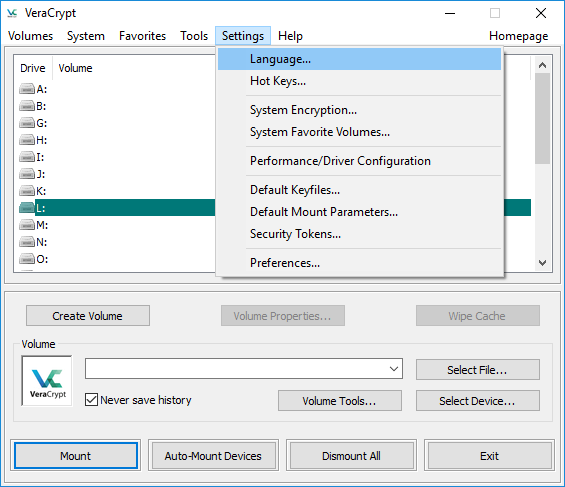
\includegraphics[width=300pt]{media/changelanguage.png}
\caption{Sprache umstellen}
\label{changelanguage}
\end{center}
\end{figure}

\newpage

\section{Einen Container erstellen}
Um einen neuen Container zu erstellen, muss zunächst der \textbf{Volume erstellen} Knopf gedrückt werden, um den Assistenten zur Erstellung von Volumen zu starten.

\begin{figure}[h]
\begin{center}
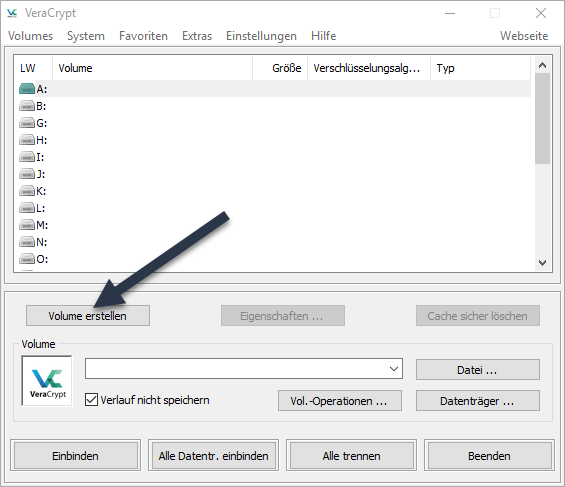
\includegraphics[width=300pt]{media/createvolumebutton.png}
\caption{Volume erstellen}
\label{createvol}
\end{center}
\end{figure}

\noindent In dem Fenster, was nun erscheint, ist standardmäßig die Option \textbf{Eine verschlüsselte Containerdatei erstellen} ausgewählt und genau diese wird jetzt auch benötigt. Dieser Schritt kann also mit dem \textbf{Weiter >} bestätigt werden.

\begin{figure}[h]
\begin{center}
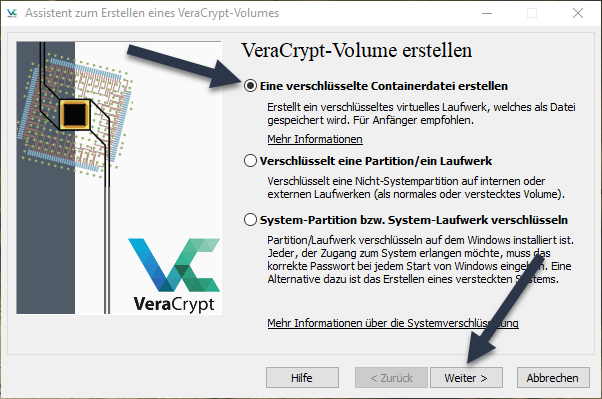
\includegraphics[width=300pt]{media/createcontainer.png}
\caption{Eine Containerdatei erstellen}
\label{createcontainer}
\end{center}
\end{figure}

\newpage

\noindent Als nächstes muss ausgewählt werden, ob die Containerdatei nur ein Standardvolumen enthalten soll, oder mit einem versteckten Volumen erstellt werden soll. Zunächst wollen wir nur einen ganz einfachen Container erstellen und lassen deshalb auch hier alles so, wie es ist.

\begin{figure}[h]
\begin{center}
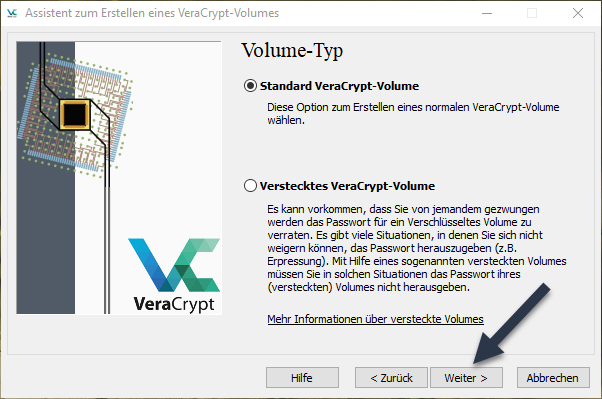
\includegraphics[width=300pt]{media/volumetype.png}
\caption{Volume-Typ}
\label{voltype}
\end{center}
\end{figure}

\noindent Nun muss ein gewünschter Dateiname gewählt werden. Endungen wie \textit{.exe} oder \textit{.dll} sind nicht zu empfehlen, da diese zu Fehlern führen können.

\begin{figure}[h]
\begin{center}
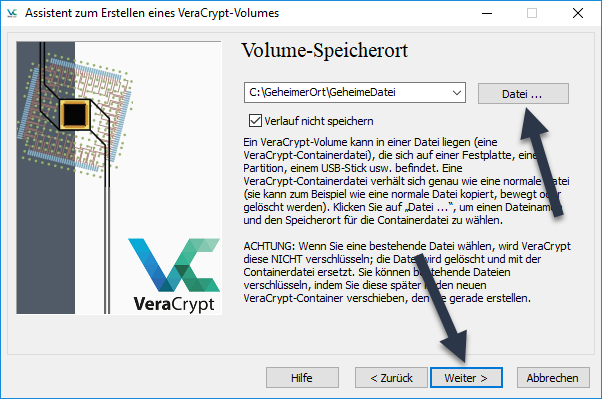
\includegraphics[width=300pt]{media/volumesavelocation.png}
\caption{Container-Speicherort}
\label{volloc}
\end{center}
\end{figure}

\newpage

\noindent Es muss jetzt ausgewählt werden, mit welchen Verschlüsselungs- und Hashalgorithmen der Container gesichert werden soll. Mehr Informationen dazu gab es bereits in Kapitel 2.3 mitsamt einer Benchmarktabelle.

\begin{figure}[h]
\begin{center}
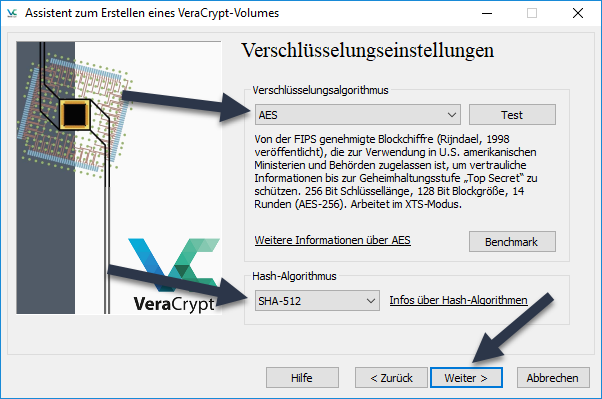
\includegraphics[width=300pt]{media/encryptionsettings.png}
\caption{Verschlüsselungseinstellungen}
\label{encryptionsettings}
\end{center}
\end{figure}

\noindent Da nun die Algorithmen gewählt wurden, kann jetzt die Dateigröße des Containers bestimmt werden. Der Container hat bereits direkt nach seiner Erstellung die gewählte Größe auf der Festplatte und wird nicht erst größer, wenn tatsächlich Dateien in dem Container liegen.

\begin{figure}[h]
\begin{center}
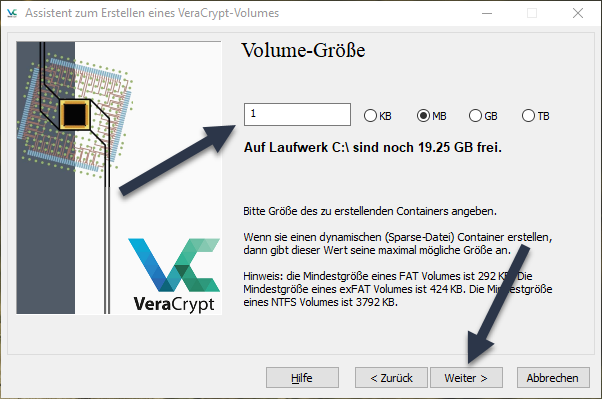
\includegraphics[width=300pt]{media/volumesize.png}
\caption{Container-Dateigröße}
\label{containersize}
\end{center}
\end{figure}

\newpage

\noindent Dieser Schritt ist der wohl wichtigste Schritt, da das verwendete Passwort die Dateien vor der Entschlüsselung schützt. VeraCrypt selbst empfiehlt eine Passwortlänge von mindestens 20 Zeichen. Weitere Informationen zur Passwortwahl liefert das Programm selbst in diesem Fenster.

\begin{figure}[h]
\begin{center}
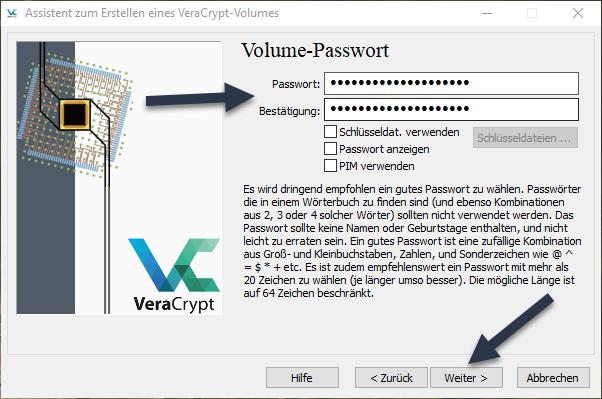
\includegraphics[width=300pt]{media/volumepassword.png}
\caption{Container-Passwort}
\label{containerpass}
\end{center}
\end{figure}

\noindent Der letzte Schritt ist die Formatierung des Containers. Sollen größere Dateien (über 4GB) im Container gespeichert werden, sollte das Dateisystem auf NTFS geändert werden. In diesem Beispiel ist es nicht möglich, da der Container gerade mal 1MB groß ist. Durch zufällige Mausbewegung innerhalb des Fensters kann zusätzliche Entropie gesammelt werden. Der Balken sollte mindestens voll sein, es schadet jedoch nicht, die Maus noch ein wenig weiter zu bewegen, bevor der Container letztendlich formatiert wird.

\begin{figure}[h]
\begin{center}
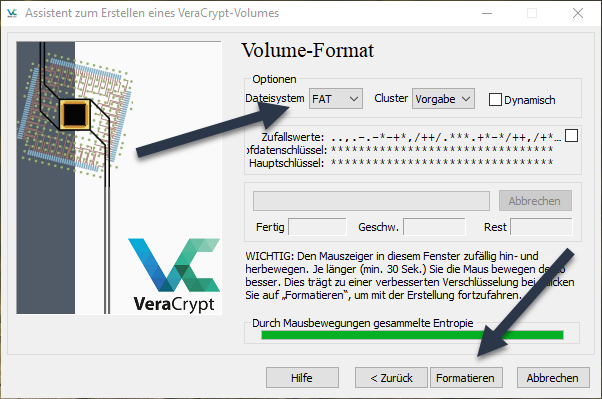
\includegraphics[width=300pt]{media/volumeformat.png}
\caption{Container-Formatierung}
\label{containerformat}
\end{center}
\end{figure}

\newpage

\section{Eine Containerdatei einbinden und trennen}

Bevor eine Containerdatei eingebunden werden kann, muss diese zunächst ausgewählt werden. Ist diese ausgewählt, kann der gewünschte Laufwerksbuchstabe in der oberen Liste ausgewählt werden und der Container mit einem Klick auf \textbf{Einbinden} eingebunden werden. Alternativ kann der Buchstabe auch doppelt angeklickt werden.

\begin{figure}[h]
\begin{center}
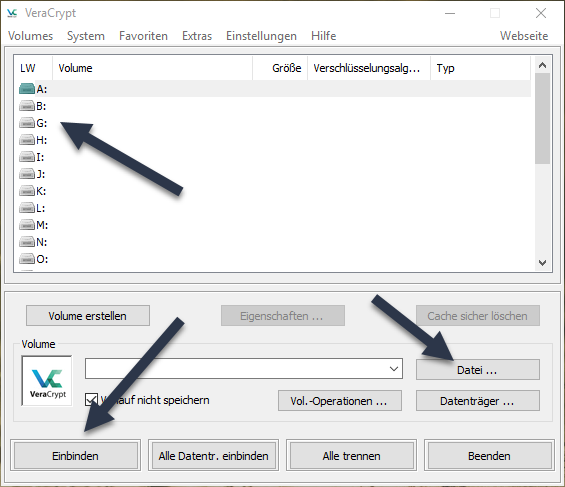
\includegraphics[width=300pt]{media/selectfile.png}
\caption{Containerdatei auswählen}
\label{selectcontainer}
\end{center}
\end{figure}

\noindent Es erscheint nun ein Dialog, in dem das zuvor gewählte Passwort eingegeben werden muss. Je nach Verschlüsselungsalgorithmus, Dateigröße und Hardware kann die Entschlüsselung sehr lange dauern.

\begin{figure}[h]
\begin{center}
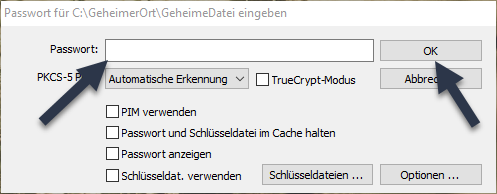
\includegraphics[width=300pt]{media/typepassword.png}
\caption{Passwort eingeben}
\label{typepassword}
\end{center}
\end{figure}

\newpage

\noindent Die Datei ist nun in Windows eingebunden und kann über den Explorer aufgerufen werden. Es reicht bereits ein Doppelklick auf den Buchstaben in VeraCrypt, um das Laufwerk direkt zu öffnen.

\begin{figure}[h]
\begin{center}
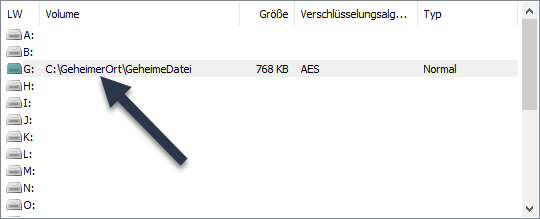
\includegraphics[width=300pt]{media/containerletter.png}
\caption{Laufwerksbuchstabe}
\label{containerletter}
\end{center}
\end{figure}

\noindent Wenn diese Datei wieder getrennt werden soll, muss der entsprechende Buchstabe per Mausklick ausgewählt werden und dann der \textbf{Trennen} Knopf gedrückt werden.

\begin{figure}[h]
\begin{center}
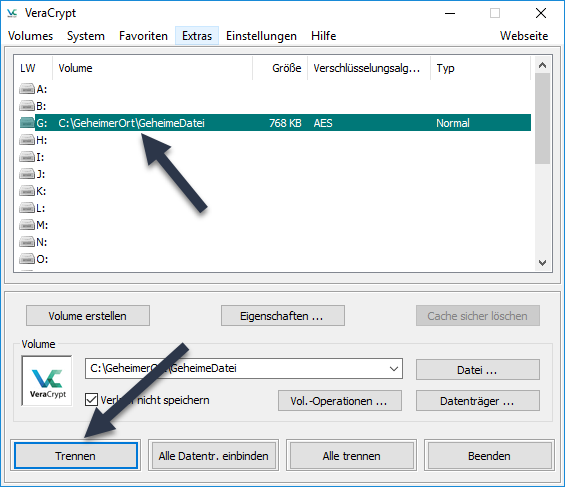
\includegraphics[width=300pt]{media/disconnectcontainer.png}
\caption{Container trennen}
\label{disconnectcontainer}
\end{center}
\end{figure}

\newpage

\section{Ein verstecktes Volume erstellen}
Die Erstellung eines versteckten Volumes ähneln der Erstellung einer normalen Volumes. Deshalb werden nur die Schritte erklärt, die neu dazu kommen. Im Gegensatz zum normalen Volume muss hier \textbf{Verstecktes VeraCrypt-Volume} ausgewählt werden.

\begin{figure}[h]
\begin{center}
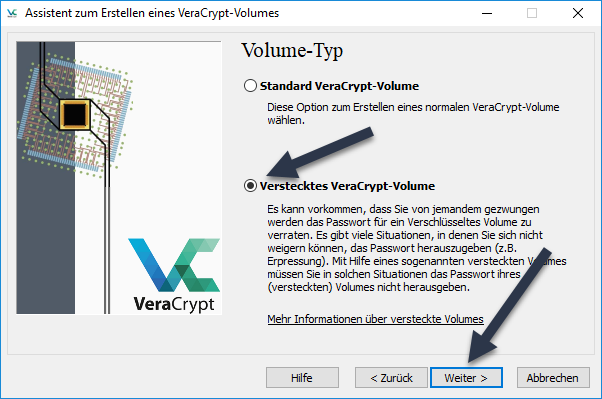
\includegraphics[width=300pt]{media/createhiddencontainer.png}
\caption{Versteckten Container erstellen}
\label{createhiddencontainer}
\end{center}
\end{figure}

\noindent Als Erstellungsmethode sollte zunächst \textbf{Kompletter Modus} gewählt werden, da hier alles auf einmal erstellt wird. Beim \textbf{Direkten Modus} kann ein verstecktes Volume innerhalb eines vorher erstelltem Volumes erschaffen werden.

\begin{figure}[h]
\begin{center}
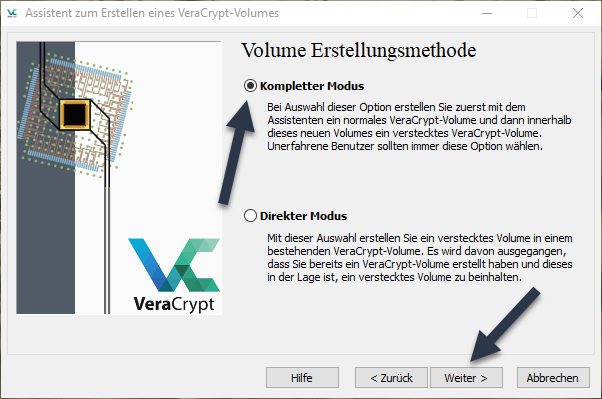
\includegraphics[width=300pt]{media/volumemode.png}
\caption{Erstellungsmethode}
\label{volumemode}
\end{center}
\end{figure}

\newpage

\noindent Zunächst wird ein einfaches Volume erstellt, in das später das versteckte Volume eingefügt wird. Wenn dieser Vorgang abgeschlossen ist, hat man die Möglichkeit das Volume mit Dateien zu füllen. Es sollte natürlich Platz gelassen werden, um das versteckte Volume zu erstellen. Diese Dateien sollten wichtig und schützenswert aussehen, damit keiner auf die Idee kommt, dass ein verstecktes Volume existiert.

\begin{figure}[h]
\begin{center}
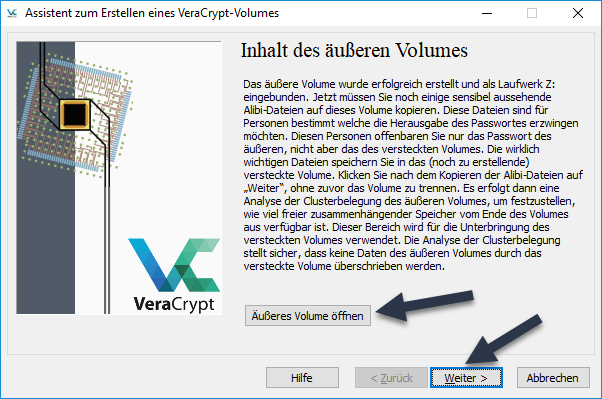
\includegraphics[width=300pt]{media/outervolume.png}
\caption{Äußeres Volume}
\label{outervolume}
\end{center}
\end{figure}

\noindent Nun können die Einstellungen für das versteckte Volume angepasst werden. Das Passwort für das versteckte Volume muss sich von dem des äußeren Volumes unterscheiden. Wenn auch das versteckte Volume erstellt wurde, ist die Datei fertig und kann eingebunden werden. Es muss bei der Einbindung einfach das Passwort des Volumes eingegeben werden, welche verwendet werden soll.\\

\noindent Wenn etwas am äußeren Volume verändert werden soll, ist es sehr zu empfehlen, das versteckte Volume zu schützen. Sollte der verfügbare Speicherplatz für das äußere Volume überschritten werden, gibt es keine Fehlermeldung, sondern das versteckte Volume wird einfach überschrieben und damit zerstört.

\begin{figure}[h]
\begin{center}
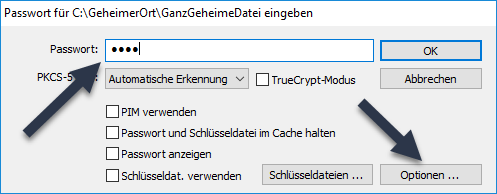
\includegraphics[width=300pt]{media/optionshidden.png}
\caption{Optionen für das versteckte Volume}
\label{optionshidden}
\end{center}
\end{figure}

\newpage

\noindent Es muss ein Haken bei \textbf{Verstecktes Volume vor Beschädigung durch äußeres Volume schützen} gesetzt werden und dann das Passwort des versteckten Volumes in der Textbox eingegeben werden. Das ganze kann mit \textbf{OK} bestätigt werden und der Container wie gewohnt eingebunden werden.

\begin{figure}[h]
\begin{center}
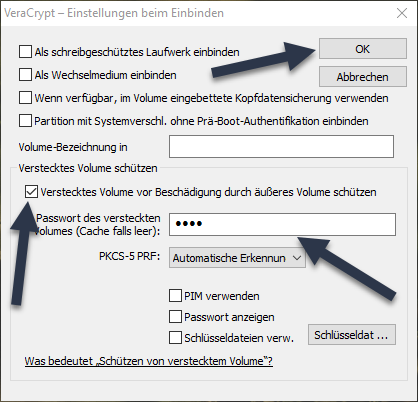
\includegraphics[width=300pt]{media/protecthidden.png}
\caption{Verstecktes Volume schützen}
\label{protecthidden}
\end{center}
\end{figure}

\newpage

\section{Eine Festplatte/USB-Stick verschlüsseln}
Um eine ganze Festplatte oder einen USB-Stick zu verschlüsseln, muss nach einem Klick auf \textbf{Volume erstellen} die zweite Option gewählt werden.

\begin{figure}[h]
\begin{center}
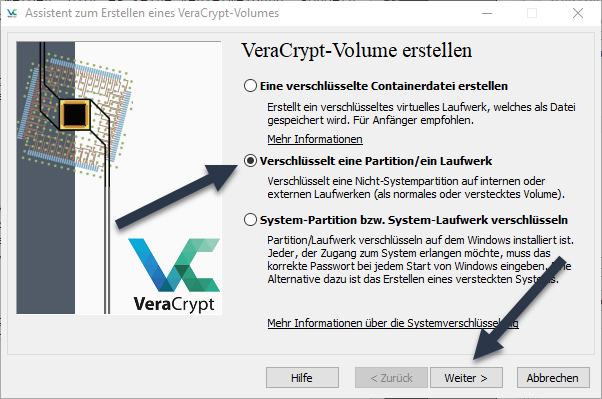
\includegraphics[width=300pt]{media/selectdeviceoption.png}
\caption{Option zur Laufwerksverschlüsselung wählen}
\label{selectdeviceoption}
\end{center}
\end{figure}

\noindent Jetzt folgt wie gewohnt die Auswahl, ob ein einfaches oder ein verstecktes Volume erstellt werden soll. Nachdem die Wahl getroffen wurde, kann der Datenträger mit einem Klick auf den \textbf{Datenträger...} Knopf ausgewählt werden. Es ist sehr wichtig keine Systempartition auszuwählen, da dies zu schwerwiegenden Fehlern führt. In diesem Beispiel handelt es sich um einen 16GB USB-Stick. Man sollte also auf eine Partition mit einer Größe in diesem Bereich achten.

\begin{figure}[h]
\begin{center}
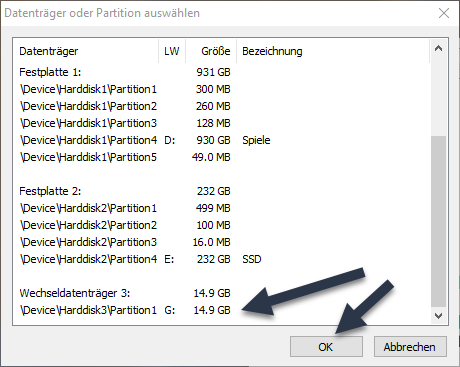
\includegraphics[width=300pt]{media/selectdevice.png}
\caption{Datenträger auswählen}
\label{selectdevice}
\end{center}
\end{figure}

\newpage

\noindent Bei dem Erstellungsmodus muss beachtet werden, ob der Stick komplett formatiert werden soll, oder ob bereits vorhandene Daten übernommen werden sollen. Befinden sich keine oder unwichtige Daten, welche ohne Probleme gelöscht werden können, auf dem Stick, so kann die Option \textbf{Verschlüsseltes Volume erstellen und formatieren} gewählt werden. Befinden sich wichtige Daten auf dem Stick, sollte die Option \textbf{Partition \glqq in-place\grqq{} verschlüsseln} gewählt werden, damit die Daten nicht verloren gehen und direkt verschlüsselt auf dem Datenträger liegen.

\begin{figure}[h]
\begin{center}
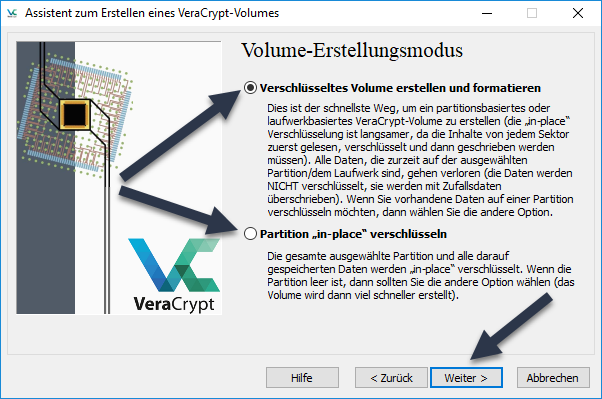
\includegraphics[width=300pt]{media/creationmode.png}
\caption{Erstellungsmodus wählen}
\label{creationmode}
\end{center}
\end{figure}

\noindent Wurde der Datenträger erfolgreich verschlüsselt, kann er im Hauptfenster über \textbf{Datenträger...} ausgewählt und danach eingebunden werden.

\begin{figure}[h]
\begin{center}
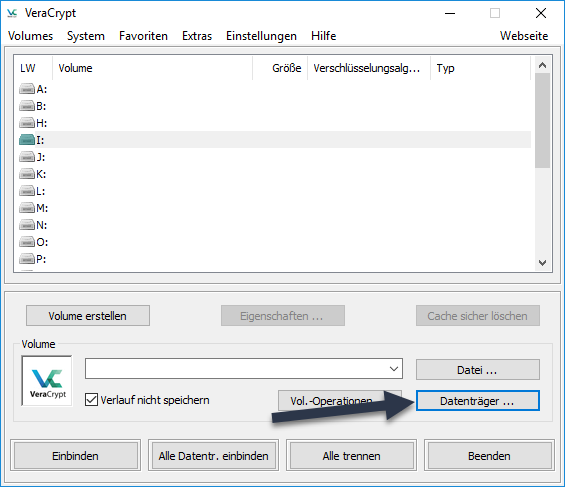
\includegraphics[width=300pt]{media/selectdevice2.png}
\caption{Datenträger auswählen}
\label{selectdevice2}
\end{center}
\end{figure}

\section{Das Betriebssystem verschlüsseln}
Das Betriebssystem zu verschlüsseln ist die sicherste Methode, da somit auch alle Verläufe und Caches mit verschlüsselt werden. Dennoch greift diese Methode sehr tief in das System ein und sollte \textbf{nur von erfahrenen Benutzern durchgeführt werden}, da VeraCrypt einen eigenen Bootloader installiert. Es sollte ein frisch installiertes System verschlüsselt werden, damit im Fall eines Fehlers keine wichtigen Daten verloren gehen.\\

\noindent Um die Prozedur zu starten, muss zunächst nach einem Klick auf den \textbf{Volume erstellen} Knopf die Option \textbf{System-Partition bzw. System-Laufwerk verschlüsseln} ausgewählt werden.

\begin{figure}[h]
\begin{center}
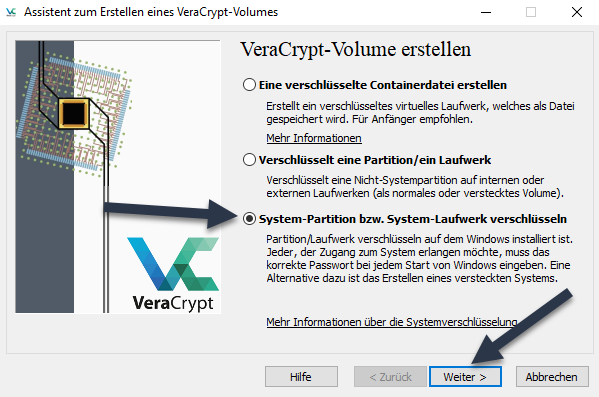
\includegraphics[width=300pt]{media/systemselection.png}
\caption{Systemverschlüsselung auswählen}
\label{systemselection}
\end{center}
\end{figure}

\noindent Nach dieser Wahl kann wieder ausgewählt werden, ob nur ein einfaches Volume oder ein verstecktes erstellt werden soll. Auch hier wird das normale gewählt, um die Anleitung kurz und verständlich zu halten, da das Prinzip der versteckten Volumes bereits erklärt wurde. Es folgt die Auswahl, welcher Bereich der Festplatte verschlüsselt werden soll. Die Option \textbf{Die Windows System-Partition verschlüsseln} sorgt dafür, dass wirklich nur die Windows Partition verschlüsselt wird, während die Option \textbf{Gesamtes Laufwerk verschlüsseln} die komplette Festplatte verschlüsselt und nur der VeraCrypt Bootloader übrig bleibt.\\

\begin{figure}[h]
\begin{center}
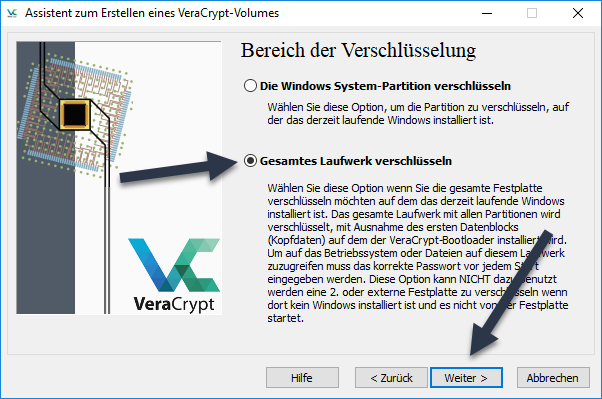
\includegraphics[width=300pt]{media/systempart.png}
\caption{Verschlüsselungsbereich auswählen}
\label{systempart}
\end{center}
\end{figure}

\newpage

\noindent Es ist nicht zu empfehlen, den geschützten Host-Bereich ebenfalls zu verschlüsseln, da auf diesem wichtige Daten des Herstellers liegen können.

\begin{figure}[h]
\begin{center}
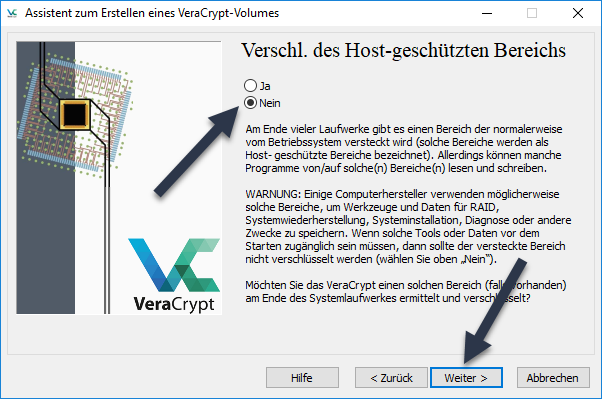
\includegraphics[width=300pt]{media/hostpart.png}
\caption{Verschlüsselung des Hostbereichs}
\label{hostpart}
\end{center}
\end{figure}

\newpage

\noindent Wenn auf dem aktuellen System nur ein Betriebssystem installiert ist, so sollte die Option \textbf{Ein Betriebssystem} gewählt werden. Ist jedoch ein Dual- oder Multiboot System mit mehreren Betriebssystem eingerichtet, muss die Option \textbf{Mehrere Betriebssysteme} ausgewählt werden.

\begin{figure}[h]
\begin{center}
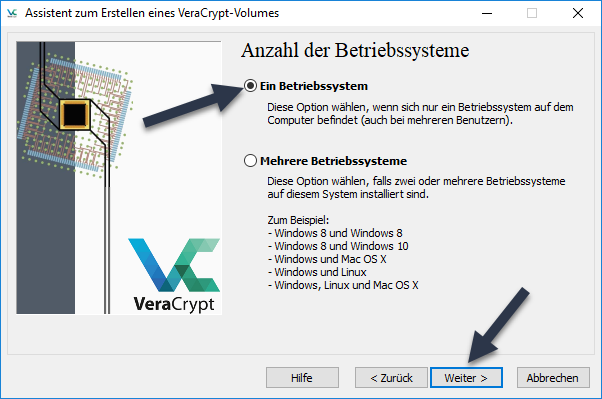
\includegraphics[width=300pt]{media/oscount.png}
\caption{Anzahl der Betriebssysteme}
\label{oscount}
\end{center}
\end{figure}

\noindent Nach den bereits bekannten Einstellung bezüglich der Verschlüsselung folgt ein Dialog, in dem die Erstellung eines Rettungsdatenträgers erfolgt. Es muss ein Ort für die Speicherung der .iso Datei gewählt werden. Es ist zu empfehlen diese Datei auf eine CD zu brennen, da sie dazu dient den Bootloader zu reparieren, falls dieser beschädigt wird. Optional kann ein Haken bei \textbf{Rettungsdatenträgerüberprüfung} gesetzt werden, um zu überprüfen, ob die Daten erfolgreich gebrannt wurden. Sollte kein Rettungsdatenträger existieren und der Booloader beschädigt werden, sind die Daten verloren, da sie nicht mehr entschlüsselt werden können.

\begin{figure}[h]
\begin{center}
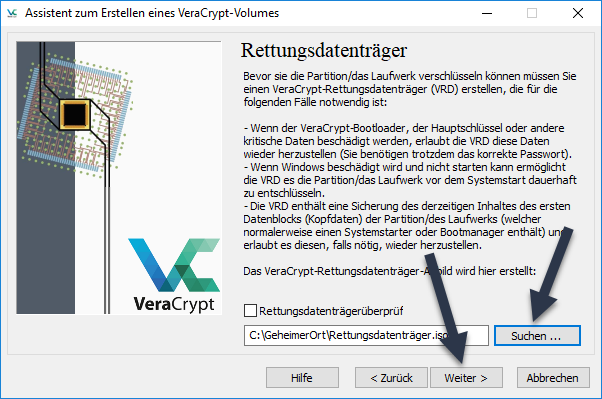
\includegraphics[width=300pt]{media/rescue1.png}
\caption{Erstellung des Rettungsdatenträgers}
\label{rescue1}
\end{center}
\end{figure}

\newpage

\noindent Es folgt eine Abfrage, wie fortgefahren werden soll. Bei der ersten Option wird lediglich die .iso Datei erstellt, die zweite Option bricht den Verschlüsselungsvorgang ab und bei der dritten Option wird die .iso Datei auf eine CD gebrannt.

\begin{figure}[h]
\begin{center}
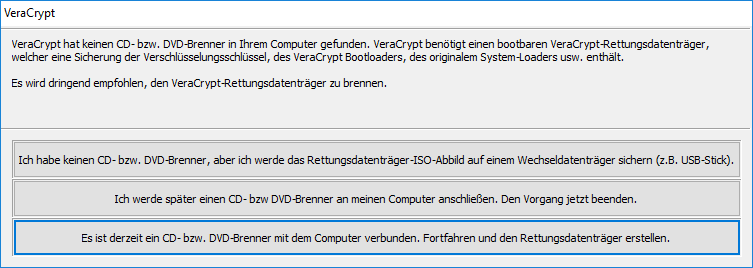
\includegraphics[width=300pt]{media/rescue2.png}
\caption{Sicherung der .iso Datei}
\label{rescue2}
\end{center}
\end{figure}

\noindent Der Löschmodus bestimmt, wie mit den vorherigen Daten umgegangen werden soll. Sollte das Risiko bestehen, dass ein Angreifer an die alten Daten gelangen möchte, sollte mindestens die Option \textbf{1-Durchgang (Zufalls Daten)} gewählt werden, damit die Rekonstruktion der Daten erschwert wird. Mehrere Durchgänge erschweren es immer weiter und können es für einen Angreifer sogar unmöglich machen die Daten wiederherzustellen.

\begin{figure}[h]
\begin{center}
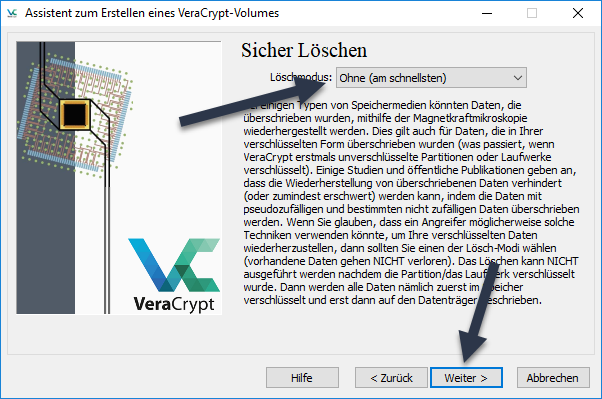
\includegraphics[width=300pt]{media/deletemode.png}
\caption{Löschmodus wählen}
\label{deletemode}
\end{center}
\end{figure}

\newpage

\noindent Es sind alle nötigen Einstellungen getroffen und es folgt ein kurzer Test, der überprüft, ob das System überhaupt mit dem VeraCrypt Bootloader zurechtkommt. Der Test kann durch einen Klick auf den \textbf{Test} Knopf gestartet werden. Bei diesem Vorgang muss der Rechner neu gestartet werden.\\

\noindent Beim Start des Systems erscheint nun der Bootloader, in dem das Passwort eingegeben werden muss. Mit der Esc Taste kann der Test auch abgebrochen werden und das System startet normal. Ist das System jedoch verschlüsselt, kann diese Abfrage natürlich nicht mehr abgebrochen werden, da sie der Entschlüsselung dient. Wie bereits in einer vorherigen Nachricht von VeraCrypt erwähnt, verwendet der Bootloader das englische Tastaturlayout, wodurch beispielsweise Anstatt einem \textit{Y} ein \textit{Z} eingegeben werden muss und anders herum.\\

\noindent Nach der Eingabe des Passworts folgt die Abfrage des PIMs. Wenn der PIM nicht spezifisch gesetzt wurde, kann einfach die Enter Taste gedrückt werden, da dies dem Standardwert entspricht.

\begin{figure}[h]
\begin{center}
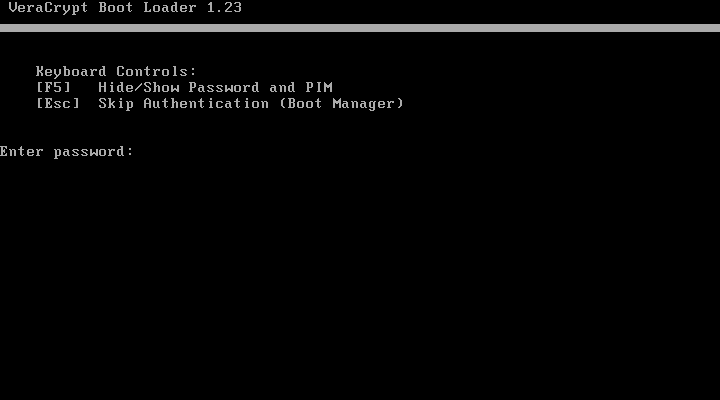
\includegraphics[width=300pt]{media/bootloader.png}
\caption{VeraCrypt Bootloader}
\label{bootloader}
\end{center}
\end{figure}

\newpage

\noindent Nachdem nun das System neu gestartet wurde, erscheint nach kurzer Zeit die Meldung, dass der Test erfolgreich war und die Verschlüsselung nun gestartet werden kann. Die Verschlüsselung kann je nach Festplattengröße, Verschlüsselungsalgorithmus und Hardwareleistung variieren. Der Rechner kann während der Verschlüsselung jedoch problemlos verwendet werden.

\begin{figure}[h]
\begin{center}
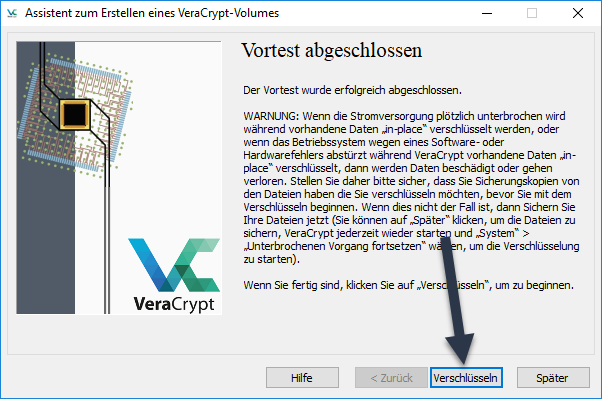
\includegraphics[width=300pt]{media/startencryption.png}
\caption{Verschlüsselung starten}
\label{startencryption}
\end{center}
\end{figure}

\noindent Nach der Verschlüsselung folgt eine kurze Meldung, dass das Laufwerk verschlüsselt wurde. Bei dem nächsten Start des System erscheint der VeraCrypt Bootloader und fragt nach dem Passwort.

\begin{figure}[h]
\begin{center}
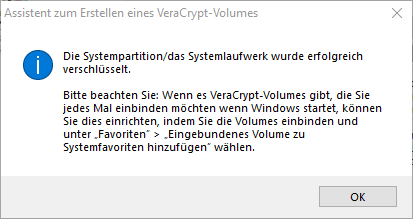
\includegraphics[width=300pt]{media/systemsuccess.png}
\caption{Verschlüsselung erfolgreich}
\label{systemsuccess}
\end{center}
\end{figure}

\newpage

\section{Das Betriebssystem dauerhaft entschlüsseln}
Sollte der Wunsch bestehen das Betriebssystem wieder in den alten Zustand zu bringen, so bietet VeraCrypt ebenfalls die Möglichkeit die Daten zu entschlüsseln. Dazu muss der \textbf{System-Partition/Laufwerk dauerhaft entschlüsseln} im \textbf{System} Menü angeklickt werden.

\begin{figure}[h]
\begin{center}
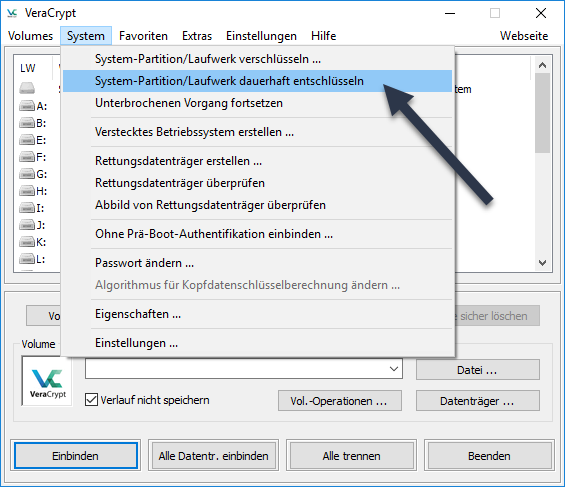
\includegraphics[width=300pt]{media/systemdecrypt1.png}
\caption{System entschlüsseln}
\label{systemdecrypt1}
\end{center}
\end{figure}

\noindent Dieser Vorgang ist sehr kurz und muss nur durch wenige Abfragen bestätigt werden. Nach der Bestätigung folgt ein Fenster, in dem der Fortschritt der Entschlüsselung zu sehen ist. Nach dem Abschluss muss das System noch einmal kurz neu gestartet werden. Das Betriebssystem ist nun komplett entschlüsselt und der Bootloader taucht nicht mehr auf.

\begin{figure}[h]
\begin{center}
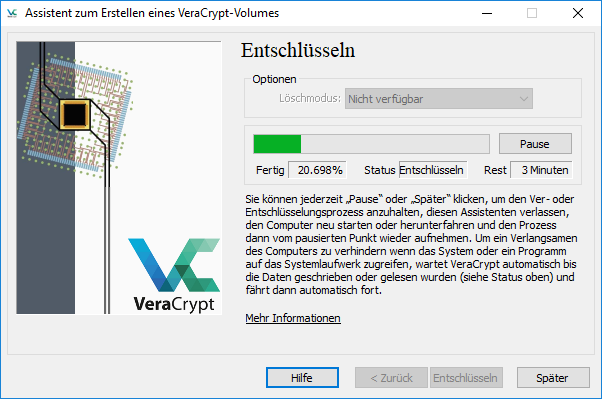
\includegraphics[width=300pt]{media/systemdecrypt2.png}
\caption{Entschlüsselungsvorgang}
\label{systemdecrypt2}
\end{center}
\end{figure}

\section{Verstecktes Betriebssystem verschlüsseln (MBR) (TODO)}
Sollte es nicht reichen, das Betriebssystem zu verschlüsseln, so muss ein verstecktes Betriebssystem her. Hierbei wird jedoch zwischen zwei Voraussetzungen unterschieden. Diese sind ein BIOS oder ein UEFI System. Um genauer so sein, MBR oder GPT.

\section{Verstecktes Betriebssystem verschlüsseln (GPD) (TODO)}

\chapter{VeraCrypt - Anhang}
Hier werden alle Informationen oder Grafiken gezeigt, die den normalen Fluss im Dokument durch ihre Größe oder Form stören würden.

\section{Benötigte Zeit um ein Passwort zu knacken}
\begin{figure}[h]
\begin{center}
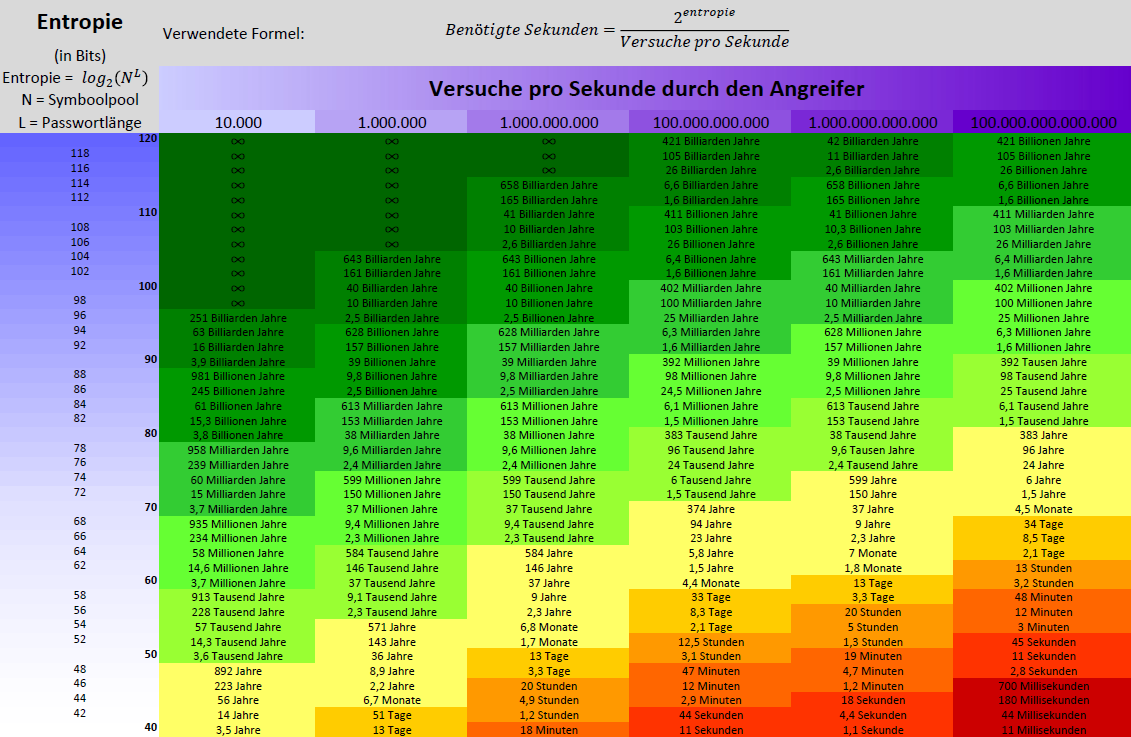
\includegraphics[width=480pt]{media/entropytable.png}
\label{entropytable}
\end{center}
\end{figure}

\part{KeePass 2}
\chapter{KeePass 2 - Theorie}
Zunächst werden die grundlegenden Prinzipien eines Passwortmanagers und einige Funktionen des Programms KeePass 2 nahegelegt. Dieser theoretische Teil ist für die Personen gedacht, die nur schnell etwas nachschlagen wollen, oder ihr Wissen gerne vertiefen. Um es kurz zu fassen, in diesem Teil zu KeePass steht alles, was für die Praxis zu lang oder kompliziert ist.

\section{Was ist KeePass?}
KeePass ist ein sogenannter Passwortmanager. Es ist eine Art verschlüsselte Datenbank in der eine Vielzahl von Passwörtern gespeichert werden kann. Das Programm liefert aber bei weitem mehr, als das simple Abspeichern und verschlüsseln von Passwörtern. Ein besonderer Punkt an KeePass ist, dass es durch Plugins erweitert werden kann und damit um Funktionen erweitert werden kann, die ein Benutzer vermisst. Ein weiterer Punkt, der für KeePass spricht ist, dass das komplette Programm und die Datenbankdatei offline verwendbar sind. Es gibt auch Alternativen, welche jedoch meistens über einen Onlinedienst laufen. Aus Sicht der Sicherheit ist es wohl doch eine bessere Idee das Passwort für die Datenbank nicht über das Internet zu verschicken, obwohl es natürlich vor der Übertragung verschlüsselt wird.
\section{Vor- und Nachteile von Passwortmanagern}
Ein Passwortmanager bietet eine Menge an Vorteilen, aber auch einige Nachteile mit sich. Ob sich der Einsatz eines Passwortmanagers lohnt, muss jeder Benutzer für sich selbst entscheiden. Was man aber mit Sicherheit sagen kann ist, dass so ein Programm das Gedächtnis deutlich entlastet. Das ist wohl mit Abstand der wichtigste Punkt bei der Verwendung eines Passwortmanagers.\\

\noindent Es wird stark empfohlen für jeden Zweck jeweils ein anderes sicheres Passwort zu verwenden. Wer sehr viel im Internet unterwegs ist, wird damit schnell überfordert sein. Außerdem wird die Komplexität der Passwörter ebenfalls nicht sonderlich hoch sein. Der klare Vorteil ist, dass quasi unendlich viele Passwörter gespeichert werden können. Der limitierende Faktor ist natürlich die Kapazität der Festplatte. Dem Benutzer kann dann aber auch die Komplexität und Länge des Passworts egal sein, da er sich nur noch ein einziges Passwort merken muss und das dient dazu, die Datenbank zu entschlüsseln. Dieses Passwort muss dann auch wirklich sehr sicher sein, damit kein Angreifer Zugriff auf alle anderen Passwörter hat.\\

\noindent Genau das ist der große Nachteil eines Passwortmanagers. Sollte die Datenbank und das Passwort bei einer böswilligen Person landen, hat diese alle Passwörter und kann damit auf jeden einzelnen Account zugreifen. Glücklicherweise bieten heutzutage viele Plattformen die Möglichkeit einer Zwei-Faktor Authentifizierung. Das bedeutet, dass nicht nur das Passwort reicht, sondern dass beispielsweise ein Bestätigungscode, welche per SMS versendet wurde, zusätzlich eingegeben werden muss.

\section{Two-Channel Auto-Type Obfuscation}
KeePass bietet die Möglichkeit einen Eintrag automatisch in einem Anmeldeformular einzutragen und den Benutzer anzumelden. Diese Funktion simuliert Tastenanschläge und sendet diese an die gewählte Anwendung. Der Nachteil daran ist, dass im schlimmsten Fall ein Keylogger auf dem System läuft und diese simulierten Tastenanschläge auslesen kann. Damit hat ein Angreifer das Passwort, selbst wenn er nicht das Masterpasswort zu der Datenbank hat.\\

\noindent Um dieses Problem zu umgehen gibt es die Methode der Two-Channel Auto-Type Obfuscation. Das Prinzip dieser Methode ist, dass das Passwort nicht komplett per Tastenanschlägen eingegeben wird, sondern Teile des Passworts in die Zwischenablage kopiert und dann eingefügt werden. Ein einfacher Keylogger kann den Zwischenspeicher nicht auslesen und ist damit keine Gefahr mehr. Es gibt jedoch auch schädliche Software, die den Zwischenspeicher auslesen kann, doch auch das ist kein großes Problem, da nur Teile des Passworts im Zwischenspeicher sind. Natürlich ist das Passwort durch diese Methode nicht komplett sicher, da es auch Schadsoftware geben kann, die beides kann und den Algorithmus hinter dieser Methoden versteht. Daher könnte diese Schadsoftware das Passwort zusammensetzen.\\

\noindent Diese sichere Methode des Auto-Type kann bei jedem Eintrag unter dem Tab \textbf{Auto-Type} durch einen Haken bei \textbf{Two-channel auto-type obfuscation} aktiviert werden.\\

\noindent Um sicher zu gehen, dass diese Methode funktioniert, sollte geprüft werden, ob die Zielanwendung die nötigen Funktionen unterstützt. Es muss möglich sein die Zwischenablage einzufügen und mit den Pfeiltasten den Cursor im Text zu bewegen.\\

\noindent Die Vorgehensweise des Algorithmus ist, dass das Passwort in zwei Teiltexte unterteilt werden. Dafür werden zufällige Zeichen aus dem Passwort genommen und damit aufgeteilt. Ein Teil wird in den Zwischenspeicher geladen und direkt in das Passwortfeld kopiert. Der Zeiger springt an den Anfang des Textes und fängt dann an die fehlenden Zeichen zu schreiben. Es wird also Beispielsweise ein Zeichen geschrieben, ein mal die rechte Pfeiltaste gedrückt, noch ein Zeichen geschrieben, drei mal nach rechts und so weiter.

\section{Verschlüsselungsalgorithmen}
Eine neue Installation von Keepass beinhaltet zwei Verschlüsselungsalgorithmen. Den Advanced Encryption Standard (AES) oder auch Rijndael-Algorithmus und den ChaCha20 Algorithmus. Beide sind Algorithmen die einen 256 Bit Schlüssel verwenden. Weitere Algorithmen können durch Plugins installiert werden, darunter auch der Serpent, Twofish oder auch der Salsa Algorithmus.

\newpage

\section{Passwort Generator Muster}

\noindent Alternativ kann eine Option bei der Generierung eines Passworts gewählt werden, die auf einem Muster basiert. Dort können bestimmte Zeichen eingegeben werden, um ein Passwort nach genau diesem Muster zu generieren.

\begin{center}
\begin{tabular}{|c|l|}
Zeichen&Resultierender Zeichensatz\\ \hline
a&abcdefghijklmnopqrstuvwxyz 0123456789\\
A&ABCDEFGHIJKLMNOPQRSTUVWXYZ abcdefghijklmnopqrstuvwxyz 0123456789\\
U&ABCDEFGHIJKLMNOPQRSTUVWXYZ 0123456789\\
d&0123456789\\
h&0123456789 abcdef\\
H&0123456789 ABCDEF\\
l&abcdefghijklmnopqrstuvwxyz\\
L&ABCDEFGHIJKLMNOPQRSTUVWXYZ abcdefghijklmnopqrstuvwxyz\\
u&ABCDEFGHIJKLMNOPQRSTUVWXYZ\\
v&aeiou\\
V&AEIOU aeiou\\
z&BCDFGHJKLMNPQRSTVWXYZ\\
Z&AEIOU\\
c&bcdfghjklmnpqrstvwxyz\\
C&BCDFGHJKLMNPQRSTVWXYZ bcdfghjklmnpqrstvwxyz\\
p&,.;:\\
b&()\big[\big]\{{}\}{}<>\\
s&\verb|!"#$%&'()*+,-./:;<=>?@[\]^_`{}~|| \\
S&A-Z a-z 0-9 \verb|!"#$%&'()*+,-./:;<=>?@[\]^_`{}~||\\
x&Hohe ANSI Symbole (U+0080 bis U+00FF)\\
\textbackslash{}\textit{x}&Ein festgelegtes Symbol. In diesem Fall immer ein x.\\
\{{}\textit{n}\}{}&Wiederholt das vorherige Symbol n mal.\\
\big[...\big]&Einen eigenen Zeichensatz definieren.\\
\end{tabular}
\end{center}

\noindent Es folgen ein paar Beispiele um die Funktionsweise der Muster zu verdeutlichen.

\begin{center}
\begin{tabular}{|l|l|}
Muster&Mögliche Ergebnisse\\\hline
ddddd&21369, 15645, 61313\\
d\{{}5\}{}&61234, 89432, 47323\\
ddlluu&43fhDS, 89djLQ, 25nrBY\\
\textbackslash{}Xdd\textbackslash{}X&X63X, X83X, X48X\\
\big[\textbackslash{}A\textbackslash{}B\textbackslash{}C\big]\{{}4\}{}&BBBC, CBAB, ABBA\\
\end{tabular}
\end{center}

\chapter{KeePass 2 - Praxis}
In diesem Kapitel werden Anleitung gezeigt, die es ermöglichen ohne viel Hintergrundwissen das Programm zu nutzen, ohne sich dabei unnötige Gedanken zu machen. Wer einen schnellen Einstieg in die Software möchte, kann die Anleitungen einfach befolgen und bei Bedarf kann im Theorie Kapitel nachgeschlagen werden.

\section{Sprache umstellen}
Um die Sprache von KeePass 2 umzustellen muss zunächst das deutsche Sprachpaket von der offiziellen Seite heruntergeladen werden. Es ist wichtig darauf zu achten, dass das Paket für die korrekte Version heruntergeladen wurde. In der heruntergeladenen .zip Datei befindet sich die Datei \textbf{German.lngx}. Diese Datei muss in den \textbf{Languages} Ordner im KeePass Installationsordner verschoben werden. Wenn die Datei in den Ordner verschoben wurde, kann KeePass gestartet und die Sprache umgestellt werden.

\begin{figure}[h]
\begin{center}
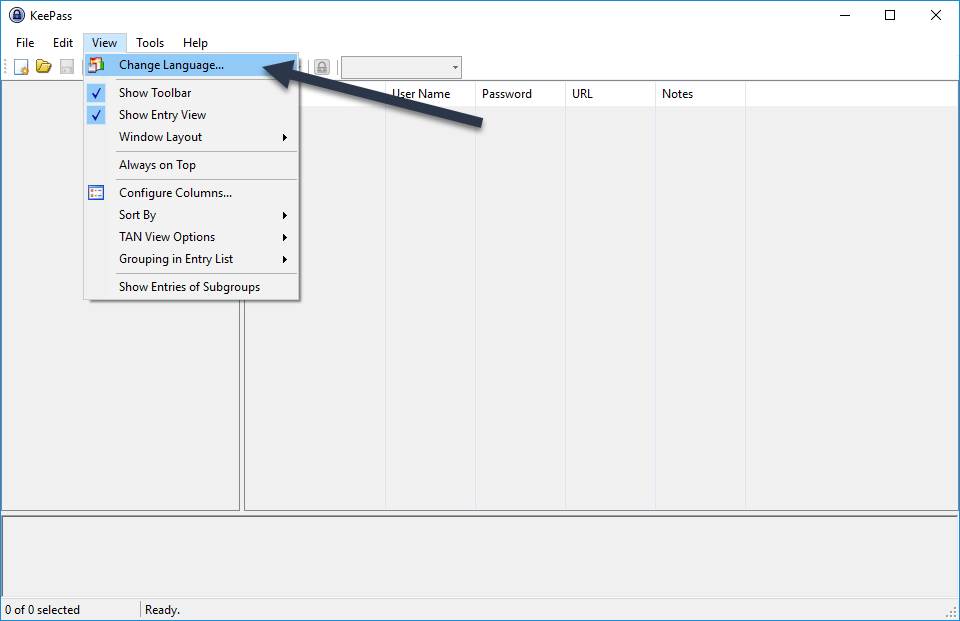
\includegraphics[width=350pt]{media/klanguage.png}
\caption{Sprache umstellen}
\label{klanguage}
\end{center}
\end{figure}

\noindent Es erscheint eine Liste mit allen verfügbaren Sprachen. Es muss nur Deutsch ausgewählt und mit einem Klick auf \textbf{OK} bestätigt werden. Das Programm muss danach neu gestartet werden. Nach dem Neustart erscheint es in der gewählten Sprache.

\newpage

\section{Eine Datenbank erstellen}
Nachdem KeePass gestartet wurde, kann eine neue Datenbank entweder mit einem Klick auf das entsprechende Symbol, oder mit der Tastenkombination \textit{Strg+N} erstellt werden.

\begin{figure}[h]
\begin{center}
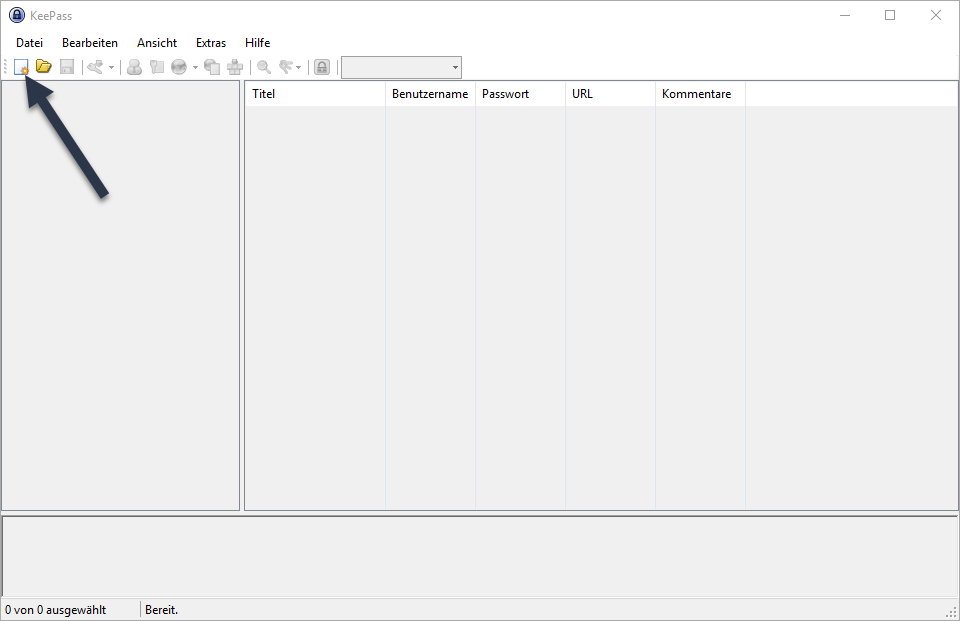
\includegraphics[width=350pt]{media/knewdb1.png}
\caption{Neue Datenbank erstellen}
\label{knewdb1}
\end{center}
\end{figure}

\noindent Es folgt ein kurzer Dialog, der einfach bestätigt werden kann. Darauf gefolgt muss der Speicherort für die Datenbankdatei gewählt werden. Als nächstes folgt die Eingabe des Passworts für die Datenbank. Dieses Passwort muss wirklich sehr stark sein, da es alle anderen Passwörter schützt. KeePass bietet auch die Möglichkeit Schlüsseldateien zu verwenden um für einen weiteren Sicherheitsfaktor zu sorgen. Außerdem kann der Windows-Benutzeraccount als Verifizierung dienen, doch davon ist eher abzuraten, da es sehr kompliziert werden kann, wenn die Datenbank auf einen anderen Rechner umziehen soll. In diesem Beispiel wird nur ein Passwort verwendet, um den Aufwand so gering wie möglich zu halten. \newpage

\begin{figure}[h]
\begin{center}
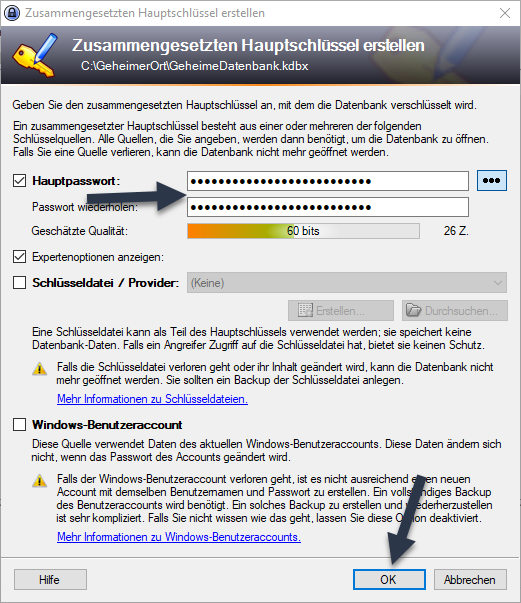
\includegraphics[width=220pt]{media/knewdb2.png}
\caption{Hauptschlüssel erstellen}
\label{knewdb2}
\end{center}
\end{figure}

\noindent Darauf folgen die Einstellungen der Datenbank. Zunächst kann ein Name und eine Beschreibung für die Datenbank gewählt werden.

\begin{figure}[h]
\begin{center}
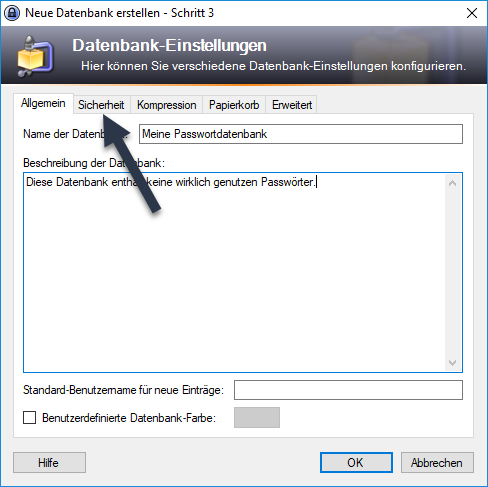
\includegraphics[width=200pt]{media/knewdb3.png}
\caption{Datenbankname und Beschreibung}
\label{knewdb3}
\end{center}
\end{figure}

\newpage

\noindent Im nächsten Tab folgt die Wahl des Verschlüsselungsalgorithmus und die Anzahl der Iterationen der Schlüsseltransformation. Es gilt dass ein Bruteforceangriff bei sehr vielen Iterationen deutlich länger dauert. Dafür dauert auch der Lade- und Speichervorgang der Datenbank dementsprechend länger.

\begin{figure}[h]
\begin{center}
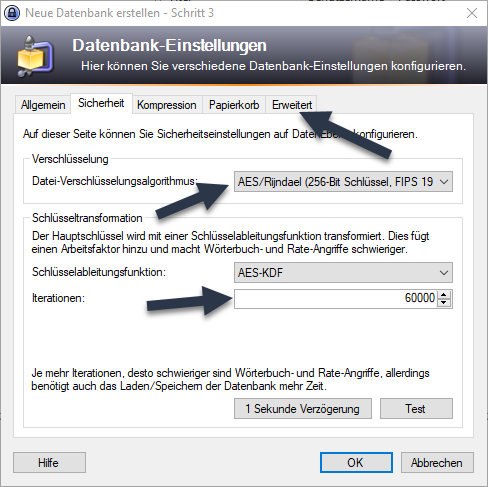
\includegraphics[width=200pt]{media/knewdb4.png}
\caption{Verschlüsselungsalgorithmus und Iterationen}
\label{knewdb4}
\end{center}
\end{figure}

\noindent Als letzter Schritt kann optional eingestellt werden, dass das Passwort für die Datenbank alle X Tage empfohlen oder erzwungen wird.

\begin{figure}[h]
\begin{center}
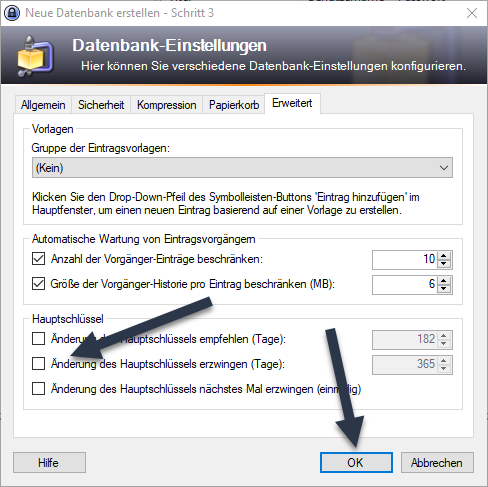
\includegraphics[width=200pt]{media/knewdb5.png}
\caption{Passwortänderung nach gewissem Zeitraum}
\label{knewdb5}
\end{center}
\end{figure}

\newpage

\noindent  Es erscheint noch ein kurzer Dialog der empfiehlt ein Notfallblatt auszudrucken. Auf diesem Notfallblatt steht der Pfad der Datenbankdatei und es kann ein Backup-Ort und das Passwort eingetragen werden. Dieses Dokument sollte natürlich sehr gut versteckt aufbewahrt, oder sogar einfach übersprungen werden.

\begin{figure}[h]
\begin{center}
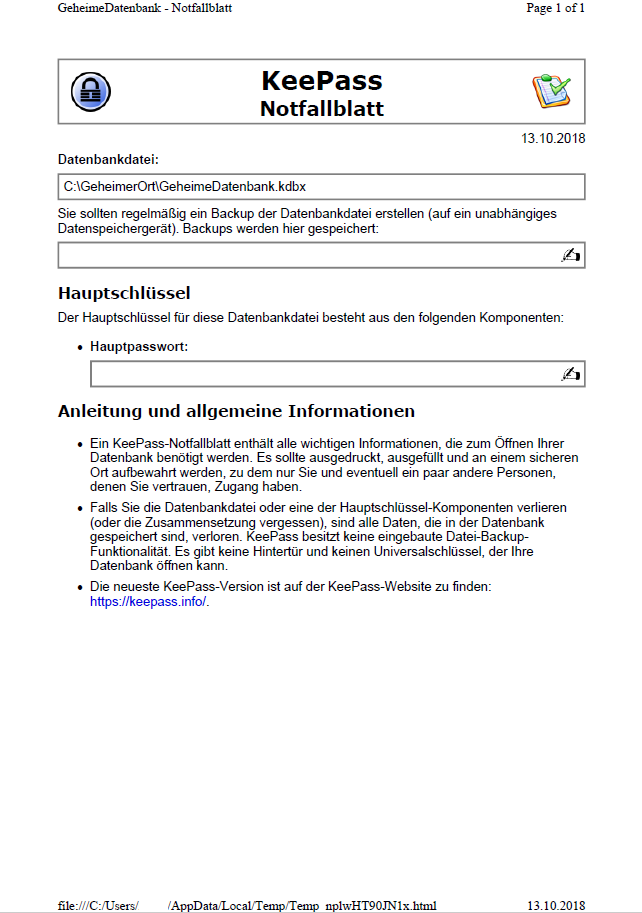
\includegraphics[width=350pt]{media/knewdb6.png}
\label{knewdb6}
\end{center}
\end{figure}

\newpage

\section{Einen Eintrag hinzufügen}
Um einen neuen Eintrag hinzuzufügen muss der Knopf mit dem Schlüsselsymbol angeklickt oder die Tastenkombination \textit{Strg+I} gedrückt werden.

\begin{figure}[h]
\begin{center}
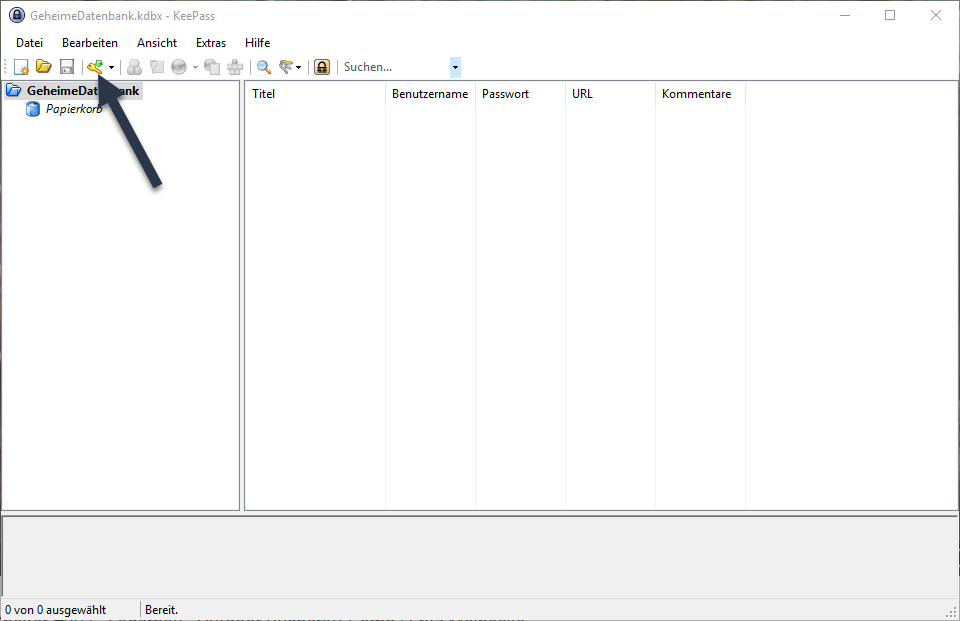
\includegraphics[width=350pt]{media/knewentry1.png}
\caption{Einen neuen Eintrag hinzufügen}
\label{knewentry1}
\end{center}
\end{figure}

\noindent Es folgt ein Fenster, in dem die wichtigsten Daten zu diesem Eintrag eingegeben werden. Zunächst der Titel, der dazu dient den Eintrag in der Liste zu identifizieren. Als Beispiel dient hier der Titel \textit{Googlemail}. Danach kann der Benutzername eingegeben werden. Alle diese Felder können natürlich auch leer gelassen werden. Nach dem Benutzernamen folgt das Passwort, das wohl wichtigste Element. Es kann entweder ein eigenes Passwort gewählt, oder der Passwort Generator verwendet werden.

\begin{figure}[h]
\begin{center}
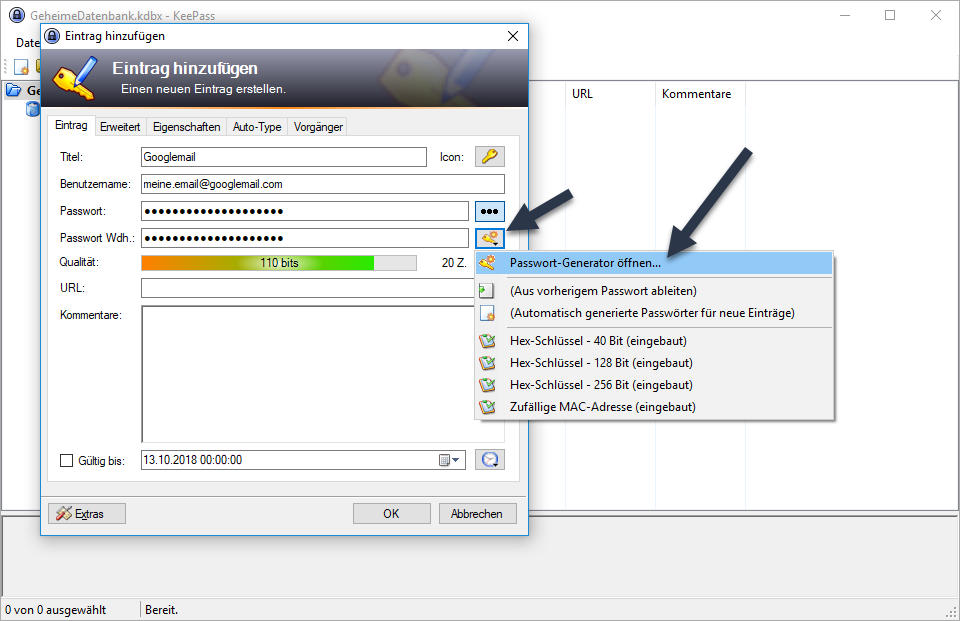
\includegraphics[width=350pt]{media/knewentry2.png}
\caption{Passwort Generator öffnen}
\label{knewentry2}
\end{center}
\end{figure}

\newpage

\noindent Der Passwort Generator ist ein mächtiges Werkzeug um ein gutes Passwort zu erstellen. Die erste Option reicht für die meisten Fälle. Es kann ausgewählt werden, wie viele Zeichen das Passwort umfassen und aus welchen Zeichen gewählt werden soll.

\begin{figure}[h]
\begin{center}
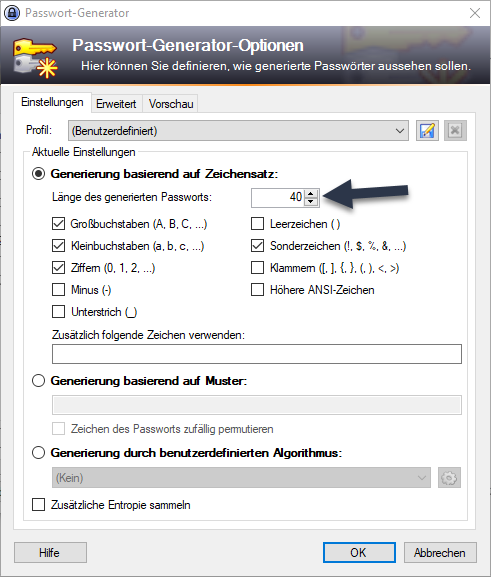
\includegraphics[width=300pt]{media/knewentry3.png}
\caption{Passwort Generator Einstellungen}
\label{knewentry3}
\end{center}
\end{figure}

\newpage



\newpage

\noindent Es kann zusätzlich noch eine URL hinterlegt werden, damit diese Website später per Tastenkombination direkt geöffnet werden kann. Als nächstes folgt der \textbf{Erweitert} Tab, denn in diesem können zusätzliche Informationen gespeichert werden, die eventuell dazu dienen, den Account wiederherzustellen, sollte er einmal verloren gehen. Damit sind alle nötigen Einstellungen getan und der Eintrag kann mit \textbf{OK} bestätigt werden.

\begin{figure}[h]
\begin{center}
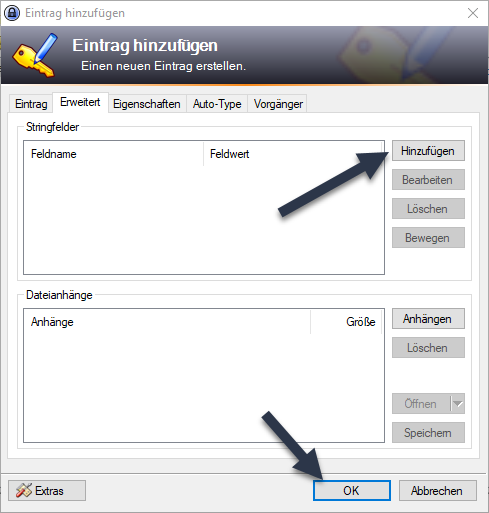
\includegraphics[width=220pt]{media/knewentry4.png}
\caption{Zusätzliche Felder}
\label{knewentry4}
\end{center}
\end{figure}

\newpage

\section{Daten kopieren und Auto-Type ausführen}
Um an die Daten eines Eintrags zu kommen muss nicht immer der Eintrag geöffnet und die Daten in den Zwischenspeicher kopiert werden. Es reicht bereits einen Doppelklick auf das entsprechende Feld zu tätigen und die Daten befinden sich für 12 Sekunden im Zwischenspeicher. Diese Limitation dient dazu, dass die Daten nicht aus Versehen in einem Textfeld landen, in dem diese nichts zu suchen haben. Alternativ können die Daten auch mit \textit{Strg+B} für den Benutzernamen und mit \textit{Strg+C} für das Passwort kopiert werden. Der Aufruf der URL erfolgt ebenfalls durch einen Doppelklick, oder durch die Tastenkombination \textit{Strg+U}.\\

\noindent Wenn Auto-Type aktiviert werden soll, so muss zunächst in das gewünschte Textfeld geklickt und dann direkt zu KeePass gewechselt werden. KeePass merkt sich das letzte Fenster, das vor KeePass aktiv war und springt bei der Aktivierung von Auto-Type in dieses Fenster. Standardmäßig sieht das Muster vom Auto-Type so aus, dass zunächst der Benutzername geschrieben wird, dann die Tabulator Taste gedrückt wird, dann das Passwort folgt und zuletzt die Eingabe mit der Enter-Taste bestätigt wird. Dieses Muster kann jedoch in den Einstellungen des Eintrags geändert werden, falls das Formular einen anderen Aufbau besitzt, oder zusätzliche Daten eingegeben werden sollen.

\begin{figure}[h]
\begin{center}
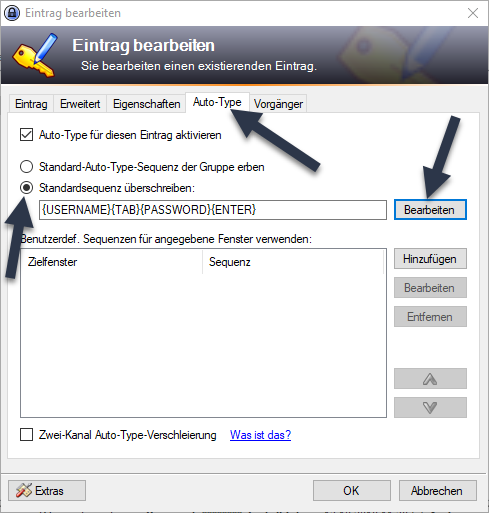
\includegraphics[width=220pt]{media/kautotype.png}
\caption{Auto-Type Muster ändern}
\label{kautotype}
\end{center}
\end{figure}

\noindent Es gibt noch eine weitere, weitaus angenehmere Variante des Auto-Type. Diese heißt globales Auto-Type, denn dafür muss nicht zunächst zu KeePass gewechselt werden. Es kann durch die Tastenkombination \textit{Strg+Alt+A} ausgeführt werden. Die Funktionsweise ist dennoch etwas anders, da hier der Titel des aktuell aktiven Fensters ausgelesen wird. KeePass sucht sich sämtliche Einträge aus, dessen Titel komplett oder teilweise im Titel des Fensters vorkommt. Sollten mehrere Einträge zu dem Titel passen, erscheint ein Dialog, aus dem der passende Eintrag ausgewählt werden kann. Die Tastenkombination für globales Auto-Type kann in den KeePass Option geändert werden.

\newpage

\section{Nützliche Einstellungen (TODO)}

\part{Paranoia Text Encryption}

\chapter{Paranoia Text Encryption - Theorie}
Bevor die Funktionsweise des Programms gezeigt wird, soll klar gemacht werden, wofür das Programm überhaupt zuständig ist. Es schadet nicht, den Theorie-Teil zu lesen, ist aber nicht nötig, um das Programm verwenden zu können. Das Programm ist ziemlich simpel, wodurch nicht viele Erklärungen nötig sind.

\section{Was ist Paranoia Text Encryption?}
Paranoia Text Encryption ist, wie es der Name bereits verrät, ein Programm mit dessen Hilfe man Text ver- und entschlüsseln kann. Der Benutzer muss ein Passwort festlegen, mit dem der Text verschlüsselt werden soll, dann den Text eingeben und das Programm verschlüsselt diesen Text dann. Der Text kann nur mit dem selben Passwort wieder entschlüsselt werden. Möchte eine andere Person den Text lesen können, so muss diese Person das Passwort kennen.

\section{Einsatzmöglichkeiten}
Das Programm eignet sich besonders gut für den Fall, wenn man einer Übertragungsmethode von Daten nicht vertraut. Das könnte beispielsweise eine einfache Email, eine SMS, oder eine Nachricht über Whatsapp sein. Selbst wenn ein Anbieter eine vollkommene Verschlüsselung verspricht, kann nur der Anbieter tatsächlich wissen, ob diese Verschlüsselung tatsächlich sicher ist, oder ob nicht doch eine Hintertür eingebaut ist. Noch schlimmer wäre es, wenn gar keine Verschlüsselung vorhanden ist. An diesem Punkt kommt Paranoia Text Encryption zum Einsatz. Mögliche Mitleser der Nachrichten können nichts mit dem Text anfangen. Nur der Sender und im Idealfall auch der Empfänger wissen, dass der Text mit diesem Programm verschlüsselt worden ist und auch noch diese Personen kennen das Passwort zur Entschlüsselung. Natürlich muss ein sicherer Weg gefunden werden, das Passwort auszutauschen. Wenn es mit gesendet wird, bringt auch die Verschlüsselung nichts.

\chapter{Paranoia Text Encryption - Praxis}
Da das Programm ziemlich leicht ist und es nur wenige, jedoch nützliche Funktionen bietet, ist das Programm sehr einfach zu überschauen. Trotzdem werden kurze Anleitungen gegeben, wie gewisse Vorgänge vollzogen werden sollten.

\section{Verschlüsselung eines Textes (TODO)}

\section{Entschlüsselung eines Textes (TODO)}

\section{Verstecken und verschlüsseln eines Textes in einem Bild (TODO)}

\section{Extrahieren und entschlüsseln eines Textes aus einem Bild (TODO)}


\part{S.S.E. File Encryptor}

\chapter{S.S.E. File Encryptor - Theorie}
Auch wenn dieses Programm noch leichter ist, als Paranoia Text Encryption, so ist eine Vorstellung und kurze Einweisung in das Programm dennoch hilfreich.

\section{Was ist S.S.E. File Encryptor?}
S.S.E. File Encryptor bietet die Möglichkeit einzelne Dateien zu verschlüsseln. Anders als bei VeraCrypt greift dieses Programm überhaupt nicht in das System ein, sondern verändert nur die betroffenen Dateien. Es muss ein Passwort angegeben werden, um eine Datei zu verschlüsseln und diese Datei kann dann nur mit diesem Passwort wieder entschlüsselt werden. Auch hier ist es eine gute zusätzliche Sicherheitsstufe, wenn eine Datei verschickt werden soll, aber dem Anbieter der Übertragungsmöglichkeit nicht vertraut wird.

\section{Sicherheitshinweise}
Es ist sehr wichtig die Datei, welche verschlüsselt wurde, sicher zu löschen, da die rohe Datei mit den richtigen Programmen wiederhergestellt werden könnte. Ein Beispiel für eine Software zur sicheren Löschung von Daten ist Eraser. Es bringt nichts eine Datei zu verschlüsseln, wenn die unverschlüsselte Version weiterhin für dritte zugänglich ist.

\chapter{S.S.E. File Encryptor - Praxis}
Das Praxiskapitel zu diesem Programm beschränkt sich lediglich auf die Ver- und Entschlüsselung von Dateien, da das Programm nicht mehr Funktionen bietet.

\section{Verschlüsselung einer Datei (TODO)}

\section{Entschlüsselung einer Datei (TODO)}

\end{document}